%++++++++++++++++++++++++++++++++++++++++
% Don't modify this section unless you know what you're doing!
\documentclass[letterpaper,12pt]{article}
\usepackage{tabularx} % extra features for tabular environment
\usepackage{amsmath}  % improve math presentation
\usepackage{authblk}  % for authors
\renewcommand\Authands{\space}
\usepackage{graphicx} % takes care of graphic including machinery
\usepackage{enumerate}
\usepackage{rotating}
\usepackage{float}
\usepackage{color}
\usepackage[margin=1in,letterpaper]{geometry} % decreases margins
\usepackage{cite} % takes care of citations
\usepackage[final]{hyperref} % adds hyper links inside the generated pdf file
\usepackage{mathrsfs}
\hypersetup{
	colorlinks=true,       % false: boxed links; true: colored links
	linkcolor=blue,        % color of internal links
	citecolor=blue,        % color of links to bibliography
	filecolor=magenta,     % color of file links
	urlcolor=blue
}
\definecolor{orange}{RGB}{255,127,0}
\newenvironment{centerverbatim}{%
  \par
  \centering
  \varwidth{\linewidth}%
  \verbatim
}{%
  \endverbatim
  \endvarwidth
  \par
}
%++++++++++++++++++++++++++++++++++++++++


\begin{document}

\title{\textbf{Charged hadron multiplicities from muon deep inelastic scattering on lH$_2$ \\ (2016 COMPASS data)}}
\author[1,2]{\textbf{N. Pierre}}
\author[3]{\textbf{M. Stolarski}}
\author[1]{\textbf{Y. Bedfer}}
\author[2]{\textbf{E. Kabu{\ss}}}
\author[1]{\textbf{F. Kunne}}
\author[ ]{\textbf{on behalf of the SIDIS group}}
\affil[1]{\textit{CEA IRFU/DPhN Saclay}}
\affil[2]{\textit{Universit\"at Mainz, Institut f\"ur Kernphysik}}
\affil[3]{\textit{LIP, Lisbon}}

\maketitle

\begin{abstract}
  We present an analysis of multiplicities of charged hadrons from 2016 data on pure proton lH$_2$ target, aiming at a release for kaons only.
  The data cover the following kinematic range : $Q^2 >$ 1 (GeV/c)$^2$, 0.1 $< y <$ 0.7, 0.004 $< x <$ 0.4,
  0.2 $< z <$ 0.85.
\end{abstract}

\newpage

\section{Introduction} \label{Intro}

In this note, we present the analysis of charged hadron multiplicities from data taken in 2016 on a pure proton lH$_2$ target, aiming at a release for kaons only.
The present release is prepared in view of the XXVII International Workshop on Deep-Inelastic Scattering and Related Subject conference in April 2019.

The new features of the present analysis, as compared to the 2006 analysis\cite{COMPASS2006P,COMPASS2006K}, are :
\begin{itemize}
	\item Data were taken on a pure proton target, compared to an isoscalar target in 2016.
	\item New Monte-Carlo simulation TGEANT.
	\item DJANGOH as Monte-Carlo event generator, taking into account radiative events at the level of event simulation\cite{DJANGOH_NOTE}.
	\item Radiative corrections as a function of z, in addition to (x,y), obtained with DJANGOH.
\end{itemize}

\section{Analysis of raw multiplicities} \label{Raw}

The analysis is performed on COMPASS data recorded in 2016 using a 160 GeV muon beam incident on a pure proton target (lH$_2$).
Five periods of the 2016 data are analyzed : P07 (slot 2), P08 (slot 2), P09 (slot 2), P10 (slot 2) and P11 (slot 2).
The whole sample has been pre-filtered into so-called μDSTs asking for at least one primary vertex with well measured beam momentum, for at least one outgoing μ with the same charge of the incoming one and for $Q^2$ $>$ 0.8 (GeV/c)$^2$. The sample with two outgoing μ was also included for a different analysis\cite{JanPt}.

The PHAST version used for this analysis is 8.001.

\subsection{Event and hadron selection}

\hfill
\newline

\textbf{DIS Selection}
\begin{enumerate}
	\item Event with a best primary vertex (PHAST routine PaEvent::iBestPrimaryVertex())
	\item Event with reconstructed scattered muon (PHAST routine PaVertex::iMuPrim())
	\item BMS cut for a well reconstructed beam track (using PaTrack::NHitsFoundInDetect("BM")$>$3)
	\item Energy of beam muon in range [140 GeV, 180 GeV]
	\item Z coordinate of event vertex ($z_{vtx}$) within the target region $\in$ [-325 cm, -71 cm]
	\item Primary interaction in the target material (PHAST routine PaAlgo:InTarget() for both data and MC (Section \ref{Raw}) target positions
				to have a complete overlap of coverage)
	\item $\chi^2$ cut for a well reconstructed beam track ($\chi^2$/ndf $<$ 10)
	\item Beam track crossing the entire target (PHAST routine PaAlgo:CrossCells())
	\item $\chi^2$ cut for a well reconstructed scattered muon track ($\chi^2$/ndf $<$ 10)
	\item Z coordinate of the first measured hit of scattered muon $<$ 350 cm ($Z_{SM1}$)
	\item Middle Trigger or Ladder Trigger or Outer Trigger or LAS trigger
	\item $Q^2$ $>$ 1 (GeV/c)$^2$
	\item 0.1 $< y <$ 0.7
	\item 5 $< W <$ 17
	\item 0.004 $< x <$ 0.4
	\item $\nu$ cut
\end{enumerate}

The cut on the kinematic variable $\nu$ was implemented to reject events that contain hadrons outside of the measured
momentum range of 12 - 40 GeV/c. The criterion is defined by :

\begin{equation}
  \nu_{max} = \frac{\sqrt{(p^2_{h,max}+m^2_h)}}{z_{max}}
\end{equation}
\begin{equation}
  \nu_{min} = \frac{\sqrt{(p^2_{h,min}+m^2_h)}}{z_{min}}
\end{equation}

where $p_{h,max}$ (resp. $p_{h,min}$) is the hadron momentum limit of 40 GeV/c (resp. 12 GeV/c), $z_{max}$ (resp. $z_{min}$)
is the upper (resp. lower) value of the $z$-bin and $m_h$ is the mass of the considered hadron.
This cut eliminates region of the ($x$,$\nu$,$z$,$p_{h}$) phase space where acceptance is zero. And consequently ($x$,$y$,$z$) acceptance correction is entirely from the LEPTO model. We thus get rid of model dependence.

\hfill
\newline

\textbf{Hadron Selection}
\begin{enumerate}
	\item Particle is not the scattered muon
	\item $\chi^2$ cut for a well reconstructed hadron track ($\chi^2$/ndf $<$ 10)
	\item Maximum radiation length cumulated along all the trajectory less than 15 radiation lengths
	\item Z coordinate of the first measured hit $<$ 350 cm ($Z_{SM1}$)
	\item Z coordinate of the last measured hit $>$ 350 cm ($Z_{SM1}$)
	\item 12 $< p_h <$ 40
	\item 0.01 $< \theta_{RICH} <$ 0.12
	\item $x^2_{RICH}+y^2_{RICH}>25$ cm$^2$
	\item 0.2 $< z <$ 0.85
\end{enumerate}

The statistics of the final data sample (5 periods) include 8.3M reconstructed DIS events and 2.6M charged hadrons.
For reference this is half the statistic of 2006.

\hspace*{0mm}\vfill
\begin{figure}[!h]
	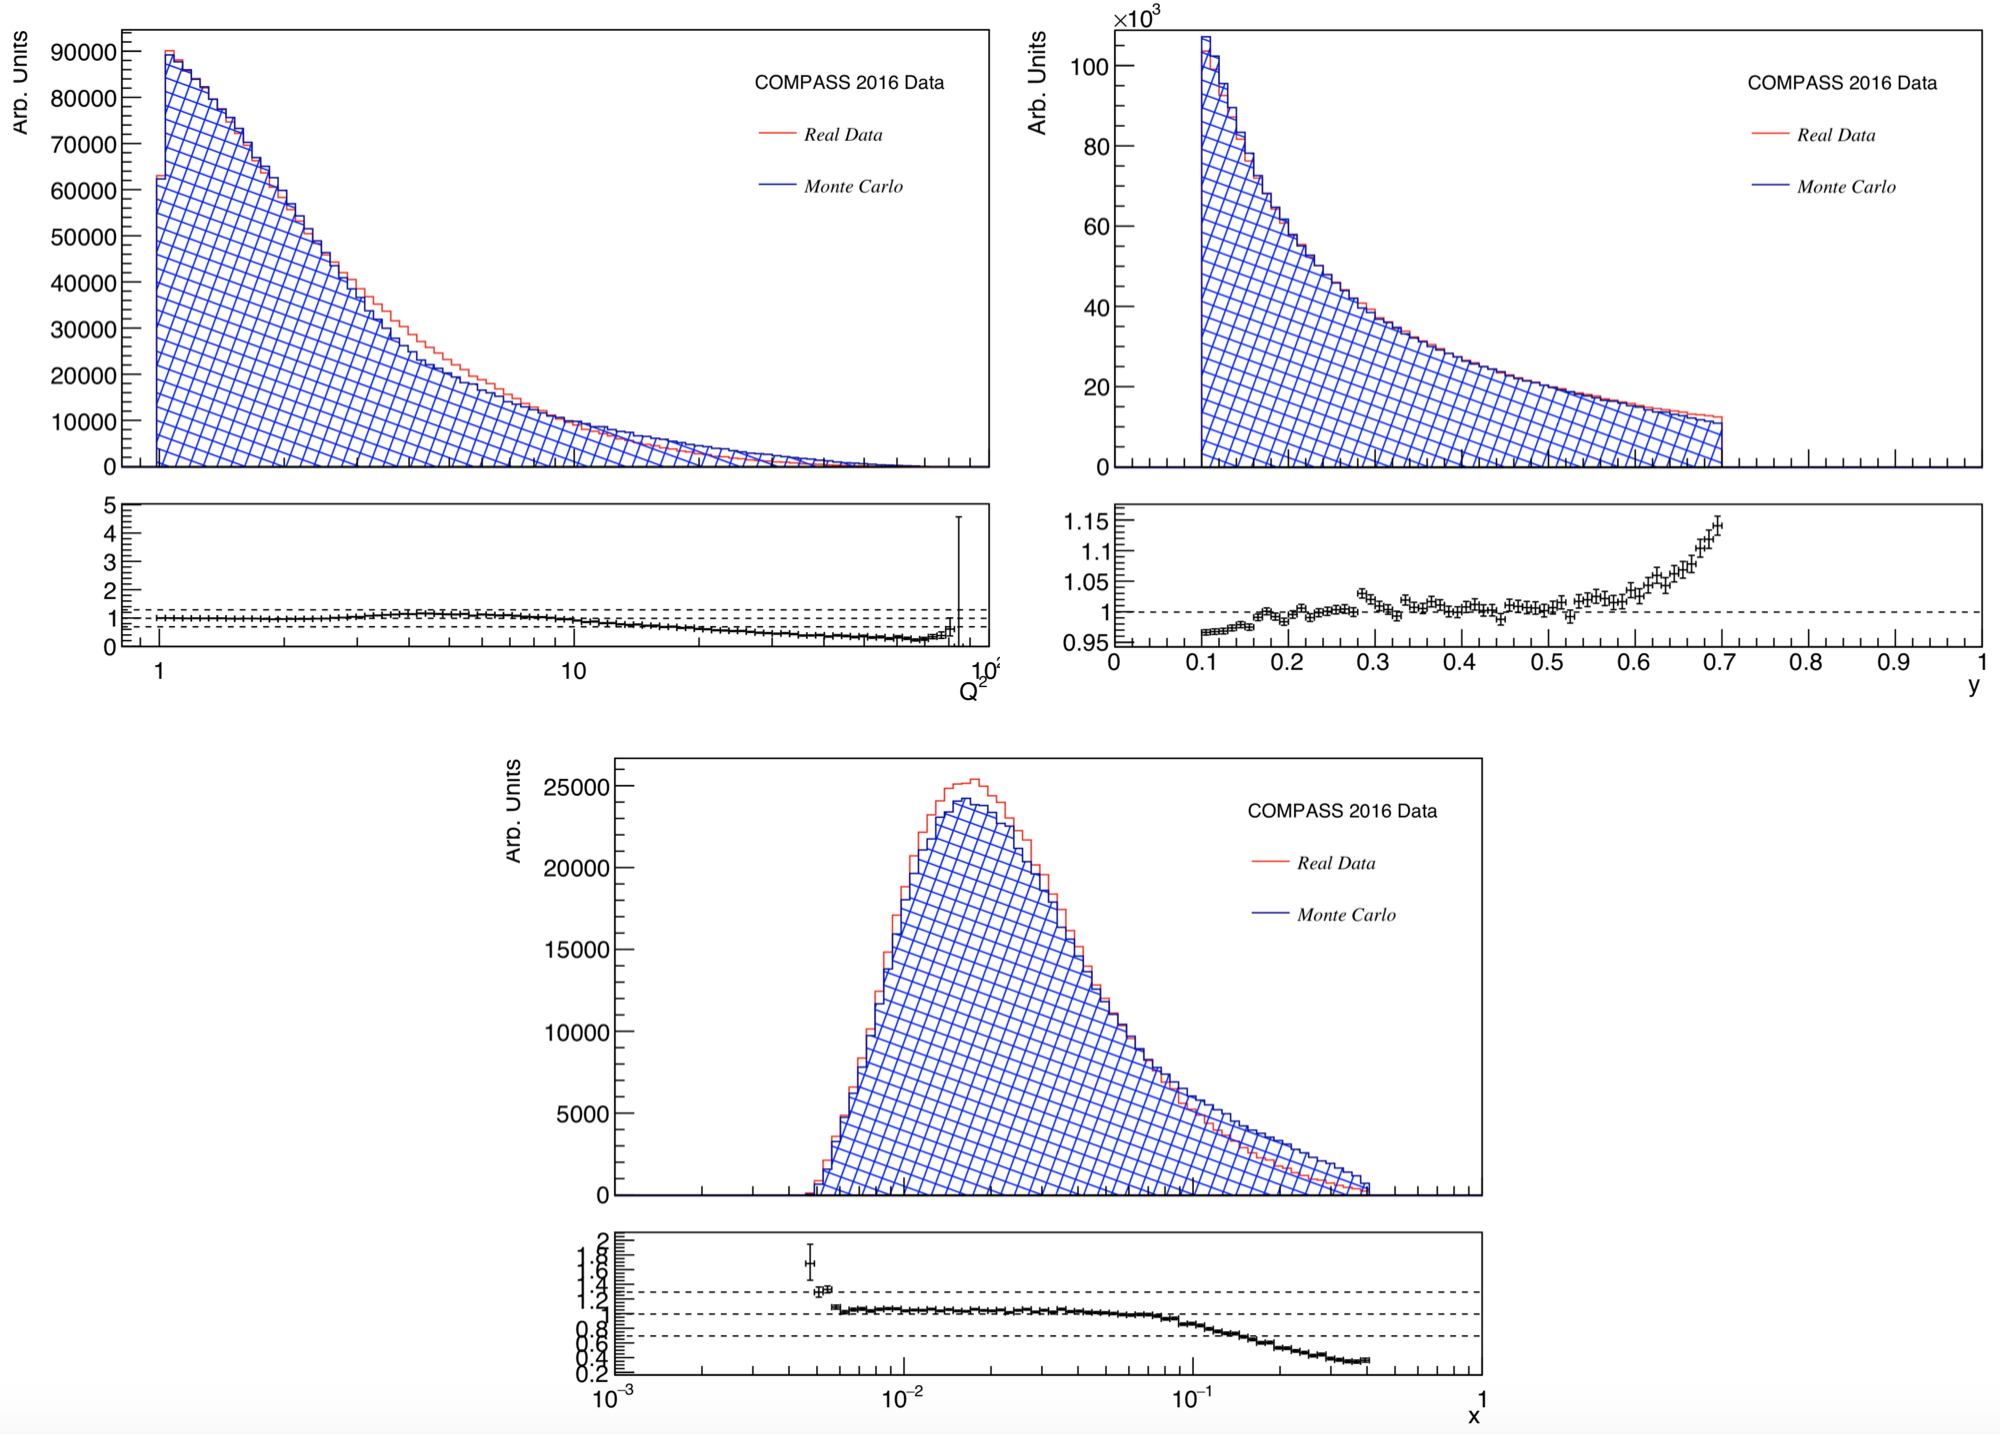
\includegraphics[scale=0.5]{./gfx/DIS_kin.png}
	\caption{Kinematical variables for DIS events ($Q^2$, $y$ and $x$) for Data (red) and Monte-Carlo (blue), as well as the ratio Data/Monte-Carlo.}
	\label{DISkin}
\end{figure}
\vfill\hspace*{0mm}

\newpage

\hspace*{0mm}\vfill
\begin{figure}[!h]
	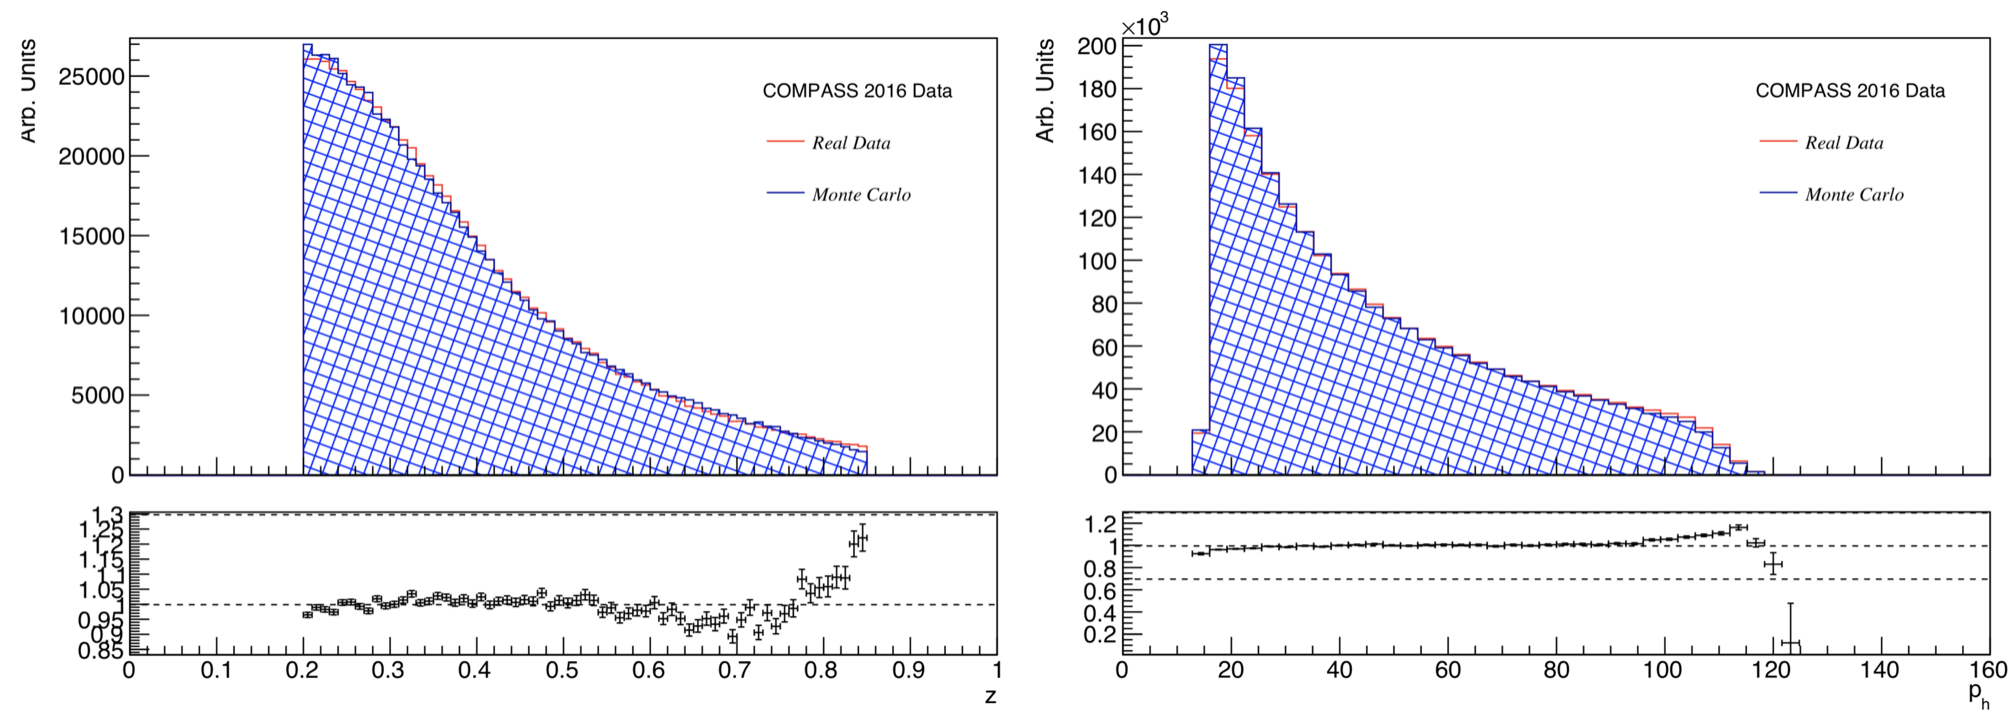
\includegraphics[scale=0.5]{./gfx/SIDIS_kin.png}
	\caption{Kinematical variables for charged hadrons ($z$ and $p_h$) for Data (red) and Monte-Carlo (blue), as well as the ratio Data/Monte-Carlo.}
	\label{SIDISkin}
\end{figure}
\vfill\hspace*{0mm}

\newpage

\subsection{Particle Identification with RICH detector}

The $\pi$, $K$ and $p$ particle identification (PID) is performed by the RICH detector.

The method used for the RICH particle identification is described in ref\cite{RICH_NOTE}. The idea is the following : when a particle
is detected, six likelihood functions are calculated ($\pi$, $K$, $p$, $e$, $\mu$ and the background) and are then
compared to make the particle identification. The evaluation is done separately for pions, kaons and protons. The largest
value corresponds to the maximal probability. The method is improved by looking further to $LH(2^{nd})$ which is the second
highest value of the four compared likelihood values ($\pi$, $K$, $p$ and the background). The electron and muon likelihood
are not considered in the assignment of $LH(2^{nd})$ as in the chosen momentum range (12 to 40 GeV/c) the RICH detector can
not be used to efficiently distinguish electrons from $\pi$.

All $\pi$, $K$ and $p$ probabilities are needed for the unfolding.

\begin{enumerate}
  \item Pion selection
  \begin{itemize}
    \item $LH(\pi) > 0$
    \item $LH(\pi) > LH(K)$, $LH(p)$ and $LH(bg)$.
    \item $\frac{LH(\pi)}{LH(2^{nd})}>1.02$
    \item $\frac{LH(\pi)}{LH(bg)}>2.02$
  \end{itemize}
  \item Kaon selection
  \begin{itemize}
    \item $LH(K) > 0$
    \item $LH(K) > LH(\pi)$, $LH(p)$ and $LH(bg)$.
    \item $\frac{LH(K)}{LH(2^{nd})}>1.08$
    \item $\frac{LH(K)}{LH(bg)}>2.08$
  \end{itemize}
  \item Proton selection
  Three cases are considered depending on the momentum $p_{h}$ of the particle and are defined but the kaon threshold ($\simeq 8.9$ GeV/c)
  and proton threshold ($\simeq 17.95$ GeV/c)
  \begin{enumerate}[(a)]
    \item Kaon threshold $< p_{h} \leq$ proton threshold - 5 GeV/c
	  \begin{center}
		  \begin{tabular}{c|c}
		    \hline
		     $p$ & $\bar{p}$ \\
		    \hline
				\multicolumn{2}{c}{Not to be a $\pi$ or $K$} \\
		    $\frac{LH(\pi)}{LH(bg)} < 2.2$ & $\frac{LH(\pi)}{LH(bg)} < 2.1$ \\
		    $\frac{LH(K)}{LH(bg)} < 2.9$ & $\frac{LH(K)}{LH(bg)} < 2.8$ \\
		    \hline
				\multicolumn{2}{c}{or all $LH$ = 0} \\
				\hline
		  \end{tabular}
		\end{center}
    \item $p_{h} >$ proton threshold + 5 GeV/c
    \begin{itemize}
      \item $LH(p) > 0$
      \item $LH(p) > LH(\pi)$, $LH(K)$ and $LH(bg)$.
      \item $\frac{LH(p)}{LH(2^{nd})}>1$
    \end{itemize}
    \item Proton threshold - 5 GeV/c $< p_{h} <$ proton threshold + 5 GeV/c
    \begin{itemize}
      \item Using (a) and (b) simultaneously.
    \end{itemize}
  \end{enumerate}
\end{enumerate}

\subsection{RICH unfolding based on efficiency matrices}

The performance of the RICH is not perfect : neither in terms of efficiency nor in terms
of purity.

The unfolding procedure is needed to correct the yield of identified hadrons for this imperfection.
In order to perform this correction, the RICH actual performance is evaluated from real data. The result of
this evaluation is presented through RICH performance matrices, $M_{RICH}$, binned in momentum
and angle :

\begin{itemize}
  \item $p_h$ \{12,13,15,17,19,22,25,27,30,35,40\} GeV/c
  \item $\theta$ \{0.01,0.04,0.12\} rad
\end{itemize}

The 3-by-3 matrices $M_{RICH}$ give a relation between the vector of true hadron $T_h$ and the vector of
identified hadron $I_h$

\begin{equation}
\begin{bmatrix}
I_{\pi} \\
I_K \\
I_p
\end{bmatrix}
=
\begin{bmatrix}
\epsilon(\pi \rightarrow \pi) & \epsilon(K \rightarrow \pi) & \epsilon(p \rightarrow \pi)\\
\epsilon(\pi \rightarrow K) & \epsilon(K \rightarrow K) & \epsilon(p \rightarrow K) \\
\epsilon(\pi \rightarrow p) & \epsilon(K \rightarrow p) & \epsilon(p \rightarrow p)
\end{bmatrix}
\begin{bmatrix}
T_{\pi} \\
T_K \\
T_p
\end{bmatrix}
\end{equation}

The coefficients of the $M_{RICH}$, $\epsilon(t \rightarrow i)$, are the probabilities that a true hadron
$t$ is identified as a hadron of type $i$. These probabilities have been determined as described in ref\cite{RICH_NOTE}.

The true hadrons have obtained by inverting the performance matrices (Eq.\ref{richmat}) :

\begin{equation}
  \overrightarrow{T_h} = M^{-1}_{RICH}\overrightarrow{I_h}
	\label{richmat}
\end{equation}

\begin{table}[!h]
  \caption{\label{HadNum} Number of identified pions, kaons, and protons for the 5 periods before and after unfolding.}
  \centering
  \begin{tabular}{lcccccc}
    \hline
     & $\pi^+$ & $\pi^-$ & $K^+$ & $K^-$ & $p$ & $\bar{p}$ \\
    \hline
    Identified & 953970 & 789480 & 253045 & 153440 & 131066 & 60705 \\
    Unfolded & 976213 & 814685 & 255132 & 150775 & 124221 & 52014 \\
    \hline
  \end{tabular}
\end{table}

\subsection{Target cut}

As the target in 2016 is long and not straight ('banana shaped'), with a shape not easily reproducible in Monte-Carlo, a combined cut on both the real data target location and the Monte-Carlo target location is performed. It is allowing us to avoid any bias concerning the target in the analysis.

\begin{figure}[!h]
	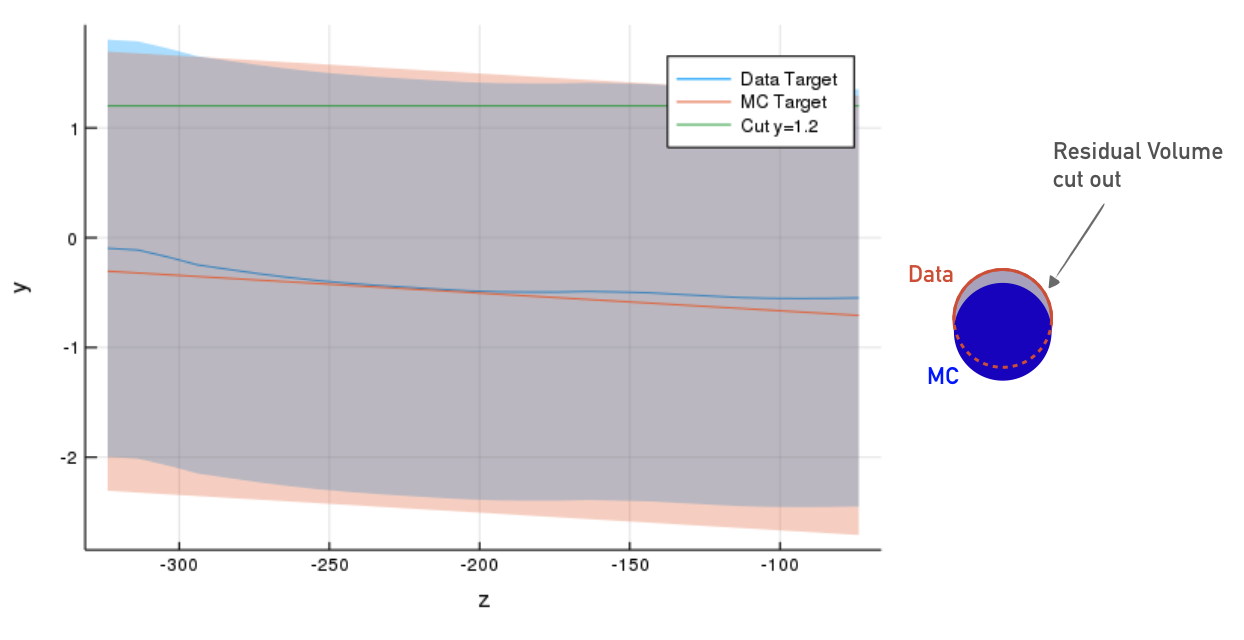
\includegraphics[scale=0.4]{./gfx/Target.png}
	\caption{Left is a ($y$,$z$) view of the real data (blue) and the Monte-Carlo target (red), $z$ being the direction of propagation of the beam. The actual cut used in the analysis corresponds to the intersection of both real data target (red) and Monte-Carlo target (blue) volumes. Right is a sketch showing approximately how much we lose by doing such cut.}
	\label{Target}
\end{figure}

\subsection{Downstream target vertex distribution}

We discovered when looking at vertex distribution for hadrons and comparing data with Monte-Carlo that there was a deficit of vertices in the downstream part of the target (between -100 and -70 cm, Fig.\ref{VertexDrop}). We saw this phenomenon both in data and Monte-Carlo however it was more stressed in data than in Monte-Carlo. After investigation, we discovered that, both in data and Monte-Carlo, there were a high number of hadrons that have their track not attached to the best primary vertex in a 2 mm-radius circle around the best primary vertex (Fig.\ref{CircleHadron}). This circle was only visible in the downstream part of the target while in the upstream part it is non-existant.

\begin{figure}[!h]
	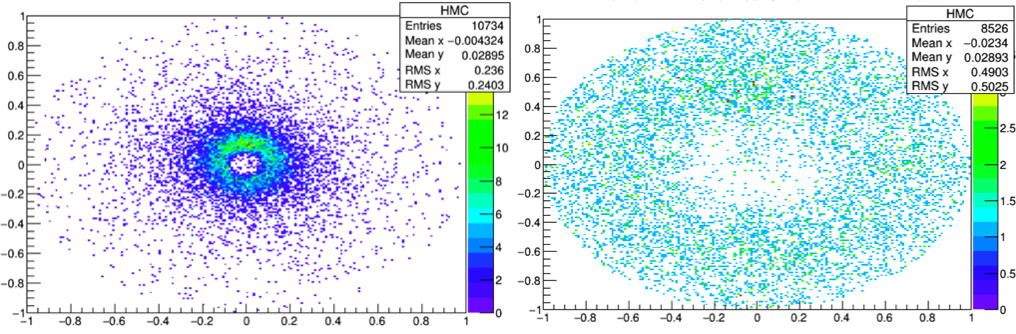
\includegraphics[scale=0.45]{./gfx/CircleHadron.png}
	\caption{Both plots are representing the relative distance to the best primary vertex of the extrapolated position of the unattached hadrons to the vertex position. Left the plot is done in the downstream part of the target, right in the upstream part. The left plot shows an important amount of particles in a 2 mm-radius circle around the vertex while the right plot does not.}
	\label{CircleHadron}
\end{figure}

This issue probably needs a thorough investigation of how the reconstruction is done in this case. As time was in short supply, we decided to go with a rescue procedure to reattach these hadrons to the best primary vertex. All the hadrons in a circle of radius 2 mm around the best primary vertex are considered as if they were attached to it (considering they have a track ID and a momentum associated). With this procedure we were able to cover for the loss of hadron in the last part of the target (Fig.\ref{VertexDrop}).

\begin{figure}[!h]
	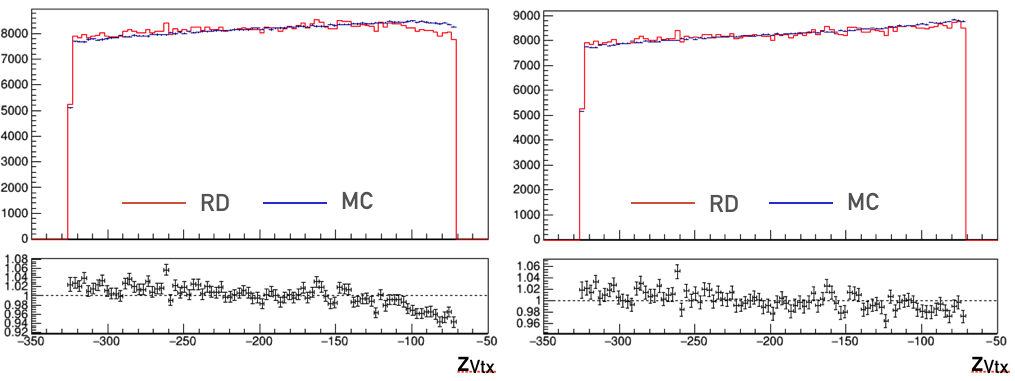
\includegraphics[scale=0.45]{./gfx/VertexDrop.png}
	\caption{One expects the vertex distribution for hadrons to increase with $z_{vtx}$ due to the apparatus acceptance. However in the left plot there is a drop both in data and Monte-Carlo of the number of vertices. In the right plot, after the rescue procedure, the drop has disappeared. The rescue procedure also reconciles data and Monte-Carlo.}
	\label{VertexDrop}
\end{figure}

\subsection{Kinematic binning}

The raw multiplicities are evaluated in bins of the Bjorken variable $x$, the muon energy fraction carried
by the virtual photon $y$ and the virtual photon energy fraction carried by final state hadron $z$. They
are calculated with the following formula :

\begin{equation}
  \frac{dM^h(x,y,z)}{dz}=\frac{1}{N^{DIS}_{Events}(x,y)}\frac{dN^{DIS}_{h}(x,y,z)}{dz}
\end{equation}

where $N^{DIS}_{Events}$ is the number of DIS events and $N^{DIS}_{h}$ is the number of
hadrons after RICH unfolding. As in practise, the multiplicities are measured in bins of
x (9 bins), y (5 bins) and z (12 bins), the calculated multiplicities can be expressed as :

\begin{equation}
  M^h_{raw}(x,y,z) = \frac{N^{DIS}_{h}(x,y,z)/\Delta z}{N^{DIS}_{Events}}
\end{equation}

where $\Delta z$ is the width of the z bin. For the multiplicities extraction, the binning in
$x$, $y$ and $z$ is the following :

\begin{itemize}
  \item $x$ \{0.004,0.01,0.02,0.03,0.04,0.06,0.1,0.14,0.18,0.4\}
  \item $y$ \{0.1,0.15,0.2,0.3,0.5,0.7\}
  \item $z$ \{0.2,0.25,0.3,0.35,0.4,0.45,0.5,0.55,0.6,0.65,0.7,0.75,0.85\}
\end{itemize}

\section{Corrections to raw multiplicities} \label{Cor}

\subsection{Detector acceptance correction}

The COMPASS detector does not cover the full phase-space then the measured multiplicities have
to be corrected for the finite detector acceptance of the order of 70\%. The correction is
done using a Monte-Carlo dataset containing about 400 million events generated in the kinematic
region $Q^2 > 0.8$ (GeV/c)$^2$, $x$ $\in$ [10$^{-4}$,0.9], $y$ $\in$ [0.01,0.95].

The events are created with DJANGOH generator with parametrization of the parton distribution functions
(MSTW08). In addition, the use of JETSET inside DJANGOH allows the hadronization of quarks q to final-state
hadrons h according to the Lund model. The COMPASS high $p_T$ tuning was used.

The same DIS event and unidentified hadron selection that are used on real data (except the BMS cut) are applied
to the MC data sample for reconstructed MC events and particles.

The data are processed through a GEANT4 model of the spectrometer, TGEANT, and events are reconstructed with the
same CORAL version as for the real data.

The acceptance involves both reconstructed and generated particles. In both cases, the particle ID is taken from
the MC truth. The following selection is made on the generated events and particles :

\begin{enumerate}
  \item Energy of the beam muon in range [140,180] GeV
	\item Z coordinate of event vertex ($z_{vtx}$) within the target region $\in$ [-325 cm, -71 cm]
	\item Primary interaction in the target material (PHAST routine PaAlgo:InTarget() for both data and MC (Section \ref{Raw}) target positions
				to have a complete overlap of coverage)
	\item Beam track crossing the entire target (PHAST routine PaAlgo:CrossCells())
  \item $Q^2>1$ (GeV/c)$^2$
  \item $0.1 < y < 0.7$
	\item $5 < W < 17$ GeV/c$^2$
  \item $0.004 < x < 0.4$
  \item $\nu$ range used in data
  \item $0.2 < z < 0.85$
\end{enumerate}

In the following, $r$ and $g$ refers to 'reconstructed' and 'generated' quantities.

The acceptance is determined as the ratio of reconstructed multiplicities $M^h_r$ over the generated multiplicities $M^h_g$
and is binned in $x$, $y$ and $z$ :

\begin{equation}
  A^h(x,y,z) = \frac{M^h_r(x,y,z)}{M^h_g(x,y,z)}=\frac{N^h_r(x,y,z)/N^{DIS}_r(x,y,z)}{N^h_g(x,y,z)/N^{DIS}_g(x,y,z)}
\end{equation}

where $x_g$, $y_g$ and $z_g$ are the generated kinematic values and $x_r$, $y_r$ and $z_r$ are the reconstructed kinematic
values.

\begin{sidewaysfigure}[!]
	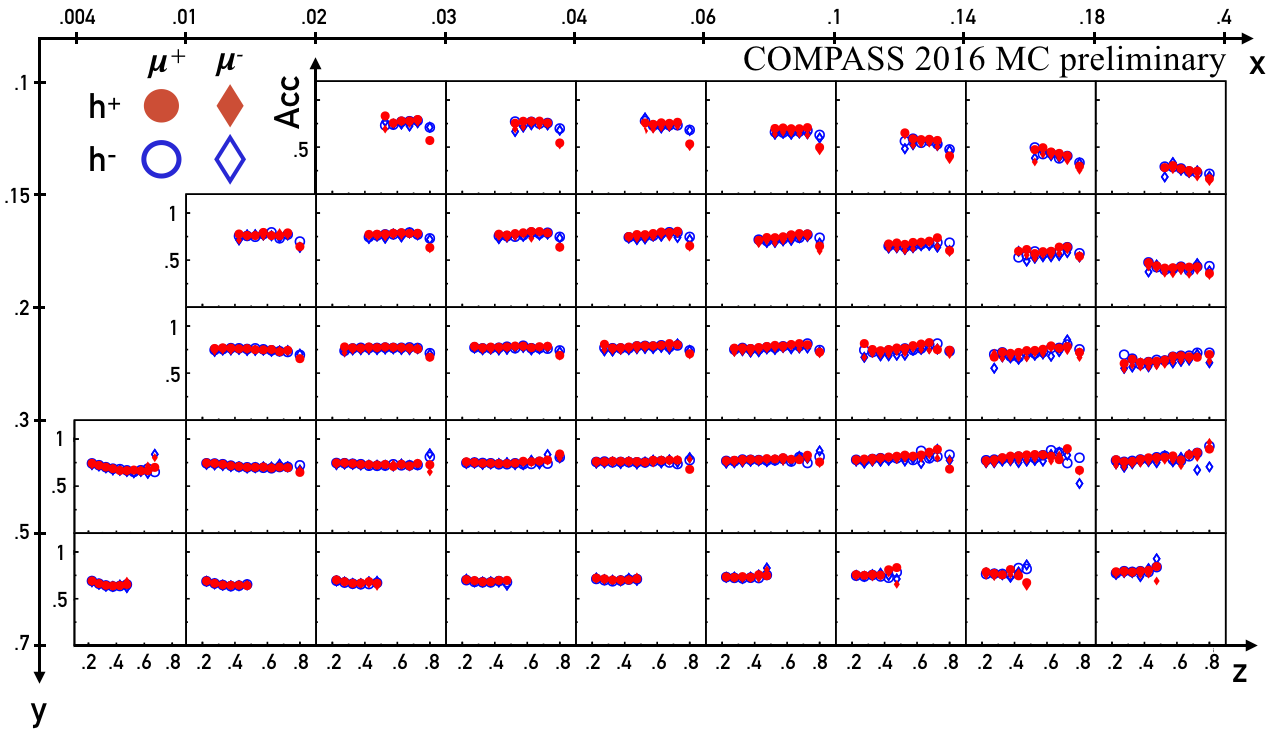
\includegraphics[scale=0.5]{./gfx/AccH.png}
	\caption{Charged hadron acceptance in $x$, $y$ and $z$ bins. The red markers correspond to positive hadrons, blue markers to negative hadrons, circles markers correspond to hadrons obtained with $\mu^+$ beam and diamonds markers to hadrons obtained with $\mu^-$ beam.}
	\label{AccH}
\end{sidewaysfigure}

\begin{sidewaysfigure}[p]
	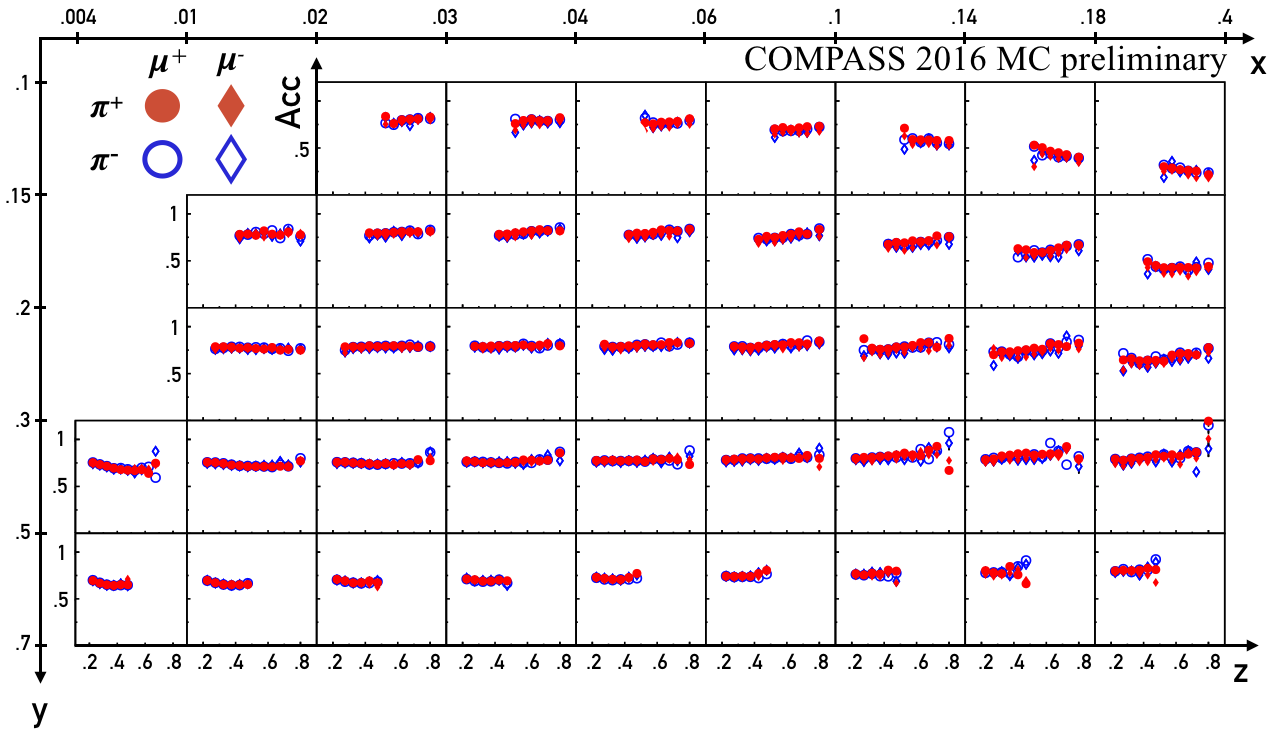
\includegraphics[scale=0.5]{./gfx/AccPi.png}
	\caption{Charged pion acceptance in $x$, $y$ and $z$ bins. The red markers correspond to positive hadrons, blue markers to negative hadrons, circles markers correspond to pions obtained with $\mu^+$ beam and diamonds markers to hadrons obtained with $\mu^-$ beam.}
	\label{AccPi}
\end{sidewaysfigure}

\begin{sidewaysfigure}[p]
	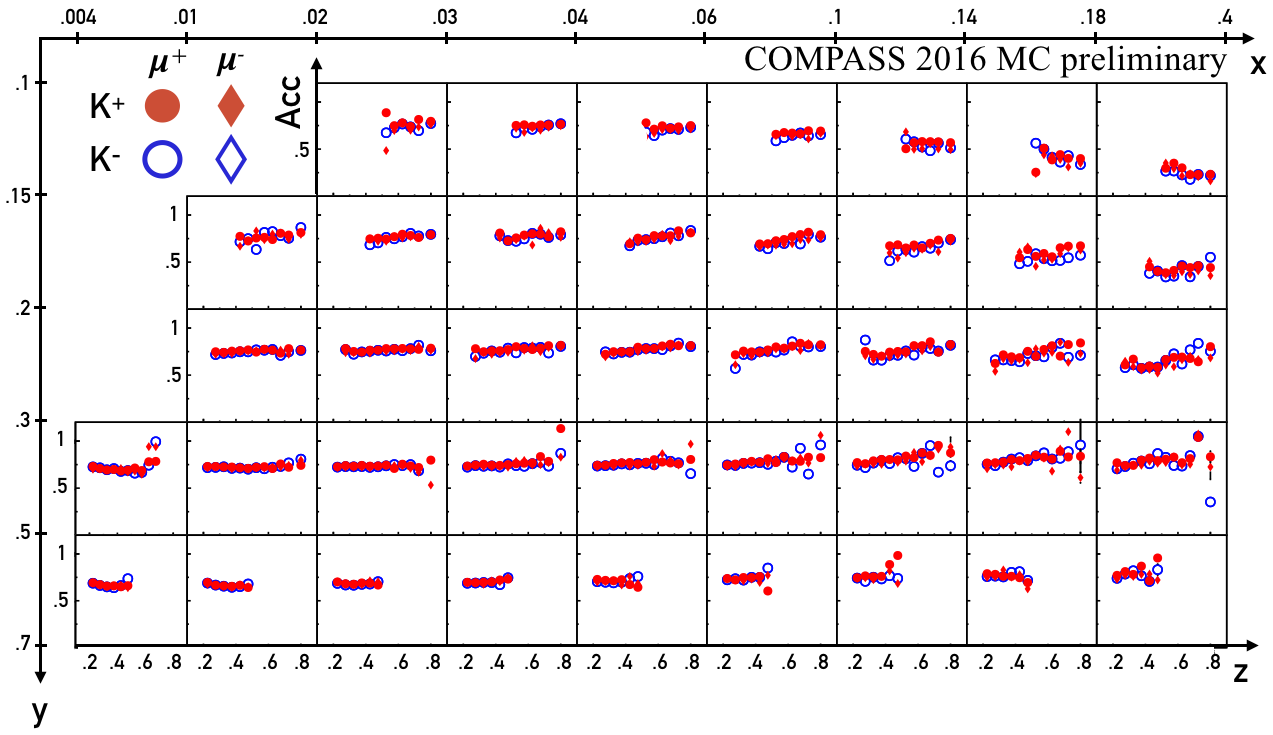
\includegraphics[scale=0.5]{./gfx/AccK.png}
	\caption{Charged kaon acceptance in $x$, $y$ and $z$ bins. The red markers correspond to positive hadrons, blue markers to negative hadrons, circles markers correspond to kaons obtained with $\mu^+$ beam and diamonds markers to hadrons obtained with $\mu^-$ beam.}
	\label{AccK}
\end{sidewaysfigure}

Used in this fashion, the kinematic bin smearing due to reconstruction limitations is accounted for. A more rigorous
bin smearing correction would involve an unfolding procedure but is not done in this analysis.

For this method, the error estimation is difficult to rigorously calculate as the numbers of evaluated hadrons and DIS events,
in both the reconstructed and generated case, are not independent. An estimation is made by considering that the hadrons numbers
and DIS events are independent of each other.

Due to the $z$ kinematic bin migration effects, there exist particles in $N_r$ which are independent from $N_g$. Decomposing $N_r$
into two independent samples namely $N_{r^0}$ which are contained in $N_g$ and $N_{r'}$ which are not, the final acceptance error yields :

\begin{equation}
  \begin{split}
    E^2_{acc} = \left (\frac{G_D}{R_D+R'_{D}}\right )^2\left [\frac{(R_h+A)(G_h-R_h+1)}{(G_h+2)^2(G_D+3)}+\frac{R'_{h}}{G^2_h}+\frac{R'^2_h}{G^3_h}\right ] \\
                + \left (\frac{G_D}{R_D+R'_{D}}\right )^4\left (\frac{R_h+R'_h}{G_h}\right )^2\left [\frac{(R_D+1)(G_D-R_D+1)}{(G_D+2)^2(G_D+3)}+\frac{R'_D}{G^2_D}+\frac{R'^2_D}{G^3_D}\right ]
  \end{split}
\end{equation}

where $G_h$ (resp. $G_D$) are the generated hadrons (resp. DIS events) in a given $x$, $y$, $z$ bin, $R_h$ (resp. $R_D$) the reconstructed
hadrons (resp. DIS events) and $R'_h$ (resp. $R'_D$) all other particles (resp. events) that are reconstructed as hadrons (resp. DIS events)
in a given $x$, $y$, $z$ bin.

The correction is then applied to the raw multiplcities :

\begin{equation}
  M^h(x,y,z) = \frac{M^h_{raw}(x,y,z)}{A^h(x,y,z)}
\end{equation}

\subsection{Diffractive vector meson correction}

It is usually assumed that hadrons produced in SIDIS originate from lepton-parton scattering. Nevertheless the scattering of a lepton
off a nucleon can also result in the diffractive production of vector mesons. These particles decay into lighter mesons that cannot be
distinguished from the one resulting from the hadronization of a quark originating from the target nucleon. This implies that fragmentation
functions extracted from multiplicities contaminated with diffractive vector mesons would violate universality, as they would be process
dependent. However, this is a complex theoretical discussion so the multiplicities both with and without subtracting the diffractive vector
meson contribution are calculated as well as the separate correction factors for DIS events and hadrons.

For kaons, the dominant vector meson contribution comes from the diffractive production of $\rho^0$ and $\Phi$ :
\begin{equation}
    \gamma * p \rightarrow \rho^0 p \rightarrow p\pi^+\pi^-
    \gamma * p \rightarrow \Phi p \rightarrow pK^+K^-
\end{equation}

This process is mainly exclusive but in 20\% of cases a diffractive dissociation of the target nucleon occurs. Other channels (excited $\rho$, $\omega$, etc.)
are expected to contribute much less and are not taken into account. As pions and kaons stemming from diffractive
vector meson decay cannot be separated from the one resulting from SIDIS, the evaluation of their contribution to the multiplicities is based on a
Monte Carlo study. Three Monte Carlo samples are produced based on different generators (SIDIS using DJANGOH, diffractive $\Phi$ using HEPGEN++) and
the same event reconstruction chain. For the diffractive vector meson samples, both exclusive events and events with diffractive dissociation of the
proton are simulated. The $\rho^0$ sample includes nuclear effects (coherent production and nuclear absorption).

The fraction of pions (resp. kaons) resulting from a diffractive $\rho^0$ (resp. $\Phi$) is calculated in the same binning as the raw multiplicities as :

\begin{equation}
  \begin{split}
    f^{\pi}_{\rho^0}(x,y,z) = \frac{N^{\pi}_{HEPGEN++}(x,y,z)}{N^{\pi}_{DJANGOH}(x,y,z)+N^{\pi}_{HEPGEN++}(x,y,z)} \\
    f^K_{\Phi}(x,y,z) = \frac{N^K_{HEPGEN++}(x,y,z)}{N^K_{DJANGOH}(x,y,z)+N^K_{HEPGEN++}(x,y,z)}
  \end{split}
\end{equation}

where $N^{\pi}_{HEPGEN++}$, $N^{\pi}_{DJANGOH}$, $N^K_{HEPGEN++}$ and $N^K_{DJANGOH}$ are the number of kaons reconstructed from the HEPGEN++ and DJANGOH MC samples normalized by the corresponding
MC luminosity ($L_{MC}$). The luminosity depends on the event weighting and the process cross-section $\sigma_{int}$ (DIS for DJANGOH event and diffractive
vector meson production for HEPGEN++ events). The final weighted number of DIS events and hadrons is summarized in Table \ref{DVM}.

\begin{equation}
  \sum_{events} w_i = L_{MC} \cdot \sigma{int}
\end{equation}

\begin{table}
	\centering
	\begin{tabular}{rccc}
    \hline
     & DJANGOH & $\rho^0$ & $\Phi$ \\
    \hline
    Generated Events & 8.4M & 19.1M & 19.2M  \\
    Weighted Generated Events & 8.4M & 280.2M & 576.9M  \\
		Integrated Cross-Section [pb] & 227010 & 12200 & 2500  \\
		Monte-Carlo Luminosity [pb$^-1$] & 36.8 & 22966.6 & 23075.2  \\
    \hline
		DIS Events [pb] & 3.4M & 96209.4 & 18083.2  \\
		$h^+$ [pb] & 630880 & 25301.9 & 3890.26  \\
		$h^-$ [pb] & 511014 & 25250.4 & 4033.93  \\
		$\pi^+$ [pb] & 453794 & 25257.4 & -  \\
		$\pi^-$ [pb] & 377335 & 25212.3 & -  \\
		$K^+$ [pb] & 102019 & - & 3872.66  \\
		$K^-$ [pb] & 75158 & - & 4015.85 \\
  \end{tabular}
  \caption{Weighted number of DIS events and hadrons for the diffractive vector meson correction. Results cross-checked with A. Moretti.}
  \label{DVM}
\end{table}

The diffractive vector meson events can also lead to a contamination in DIS events. Here, the two channels studied are diffractive $\rho^0$ and $\Phi$
with the fraction of the contamination expressed in Eqs. 13. Contrary to previous Eq. 11, the denominator only includes the DIS events from the
DJANGOH generator because the cross-section used to generate the DJANGOH sample takes into account the diffractive contribution.

\begin{sidewaysfigure}[!]
	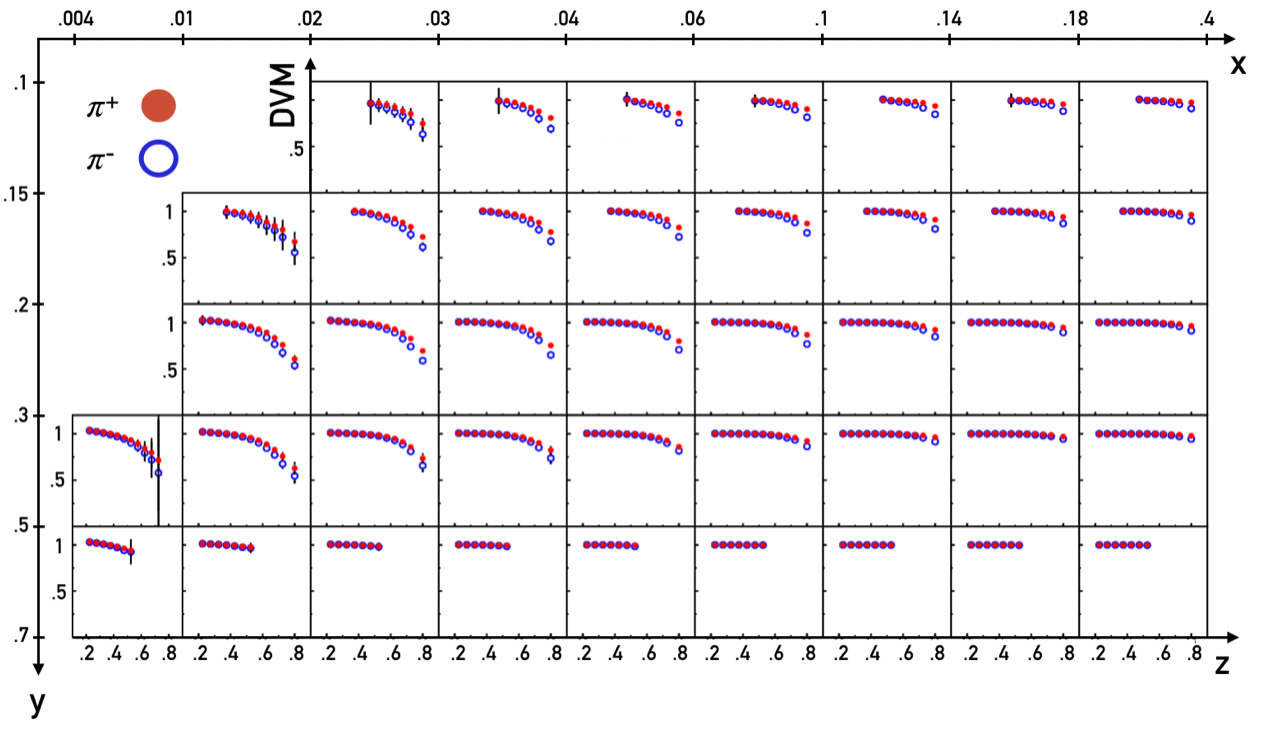
\includegraphics[scale=0.5]{./gfx/DVMpi.png}
	\caption{Correction factor $B^{\pi}$ for diffractive vector meson contamination as a function of $z$ for ($x$,$y$) bins. The red markers correspond to positive pions and blue markers for negative pions.}
	\label{DVMpi}
\end{sidewaysfigure}

\begin{sidewaysfigure}[!]
	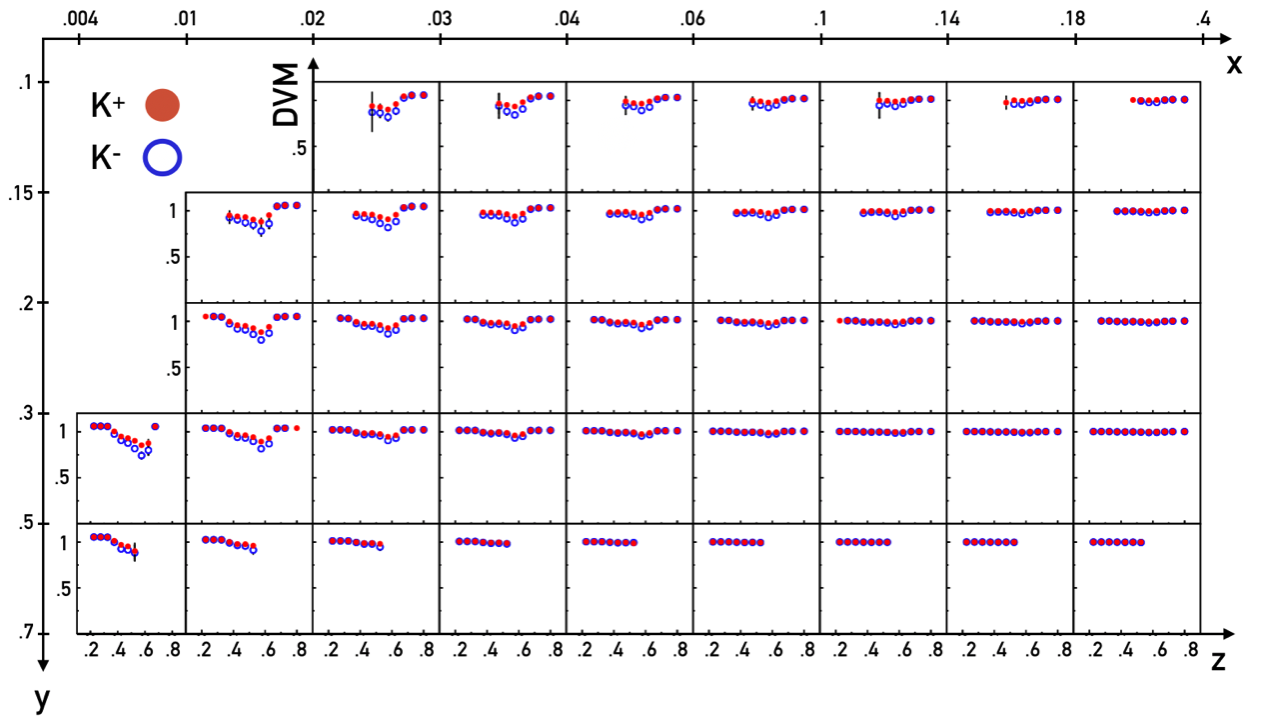
\includegraphics[scale=0.5]{./gfx/DVMK.png}
	\caption{Correction factor $B^{K}$ for diffractive vector meson contamination as a function of $z$ for ($x$,$y$) bins. The red markers correspond to positive kaons and blue markers for negative kaons.}
	\label{DVMK}
\end{sidewaysfigure}

\begin{equation}
  \begin{split}
    f^{\rho^0}_{DIS}(x,y,z) = \frac{N^{DIS}_{\rho^0,HEPGEN++}(x,y,z)}{N^{DIS}_{DJANGOH}(x,y,z)+N^{DIS}_{\rho^0,HEPGEN++}(x,y,z)+N^{DIS}_{\Phi,HEPGEN++}(x,y,z)} \\
    f^{\Phi}_{DIS}(x,y,z) = \frac{N^{DIS}_{\Phi,HEPGEN++}(x,y,z)}{N^{DIS}_{DJANGOH}(x,y,z)+N^{DIS}_{\rho^0,HEPGEN++}(x,y,z)+N^{DIS}_{\Phi,HEPGEN++}(x,y,z)}
  \end{split}
\end{equation}

The total contribution from the diffractive vector-meson contribution ($f^{VM}_{DIS}$) to the DIS sample is the sum of the $f^{\rho^0}_{DIS}$ and $f^{\Phi}_{DIS}$.
The final correction reads as follows :

\begin{equation}
  \begin{split}
  B^h(x,y,z) = \frac{ \frac{N^{\pi}(x,y,z)}{N^h(x,y,z)}\left (1-f^{\pi}_{\rho^0}(x,y,z)\right )
                   + \frac{N^K(x,y,z)}{N^h(x,y,z)}\left (1-f^{K}_{\Phi}(x,y,z)\right ) + \frac{N^p(x,y,z)}{N^h(x,y,z)} }{1-f^{VM}_{DIS}(x,y,z)} \\
  B^{\pi}(x,y,z) = \frac{1-f^{\pi}_{\rho^0}(x,y,z)}{1-f^{VM}_{DIS}(x,y,z)} \\
  B^K(x,y,z) = \frac{1-f^{K}_{\Phi}(x,y,z)}{1-f^{VM}_{DIS}(x,y,z)}
  \end{split}
\end{equation}

\subsection{Radiative corrections}

The experimental multiplicities are affected by QED radiative effects, which introduces a systematic bias of the measured kinematics with respect to the true kinematics. The most important contributions at first order are the initial and final state radiation of a real photon by the incoming or outgoing lepton. The correction factor used to take into account these phenomena is the radiative correction factor defined as :

\begin{equation}
	\eta(x,y,z) = \frac{d^2 M_{1\gamma}/dxdydz}{d^2 M_{measured}/dxdydz}
\end{equation}

where $M_{1\gamma}$ denotes multiplicities obtained using the cross-section in the one photon exchange approximation and $M_{measured}$ denotes multiplicities obtained using the measured cross-section which includes radiative effects. The bias on the $\mu$ kinematics upon real photon emission affects in turn the reconstruction of the hadron energy fraction $z$. This effect is now taken into account thanks to DJANGOH. In this analysis, the multiplicities are directly corrected. Fig.\ref{RadCor} shows the effect of the correction.

\begin{sidewaysfigure}[!]
	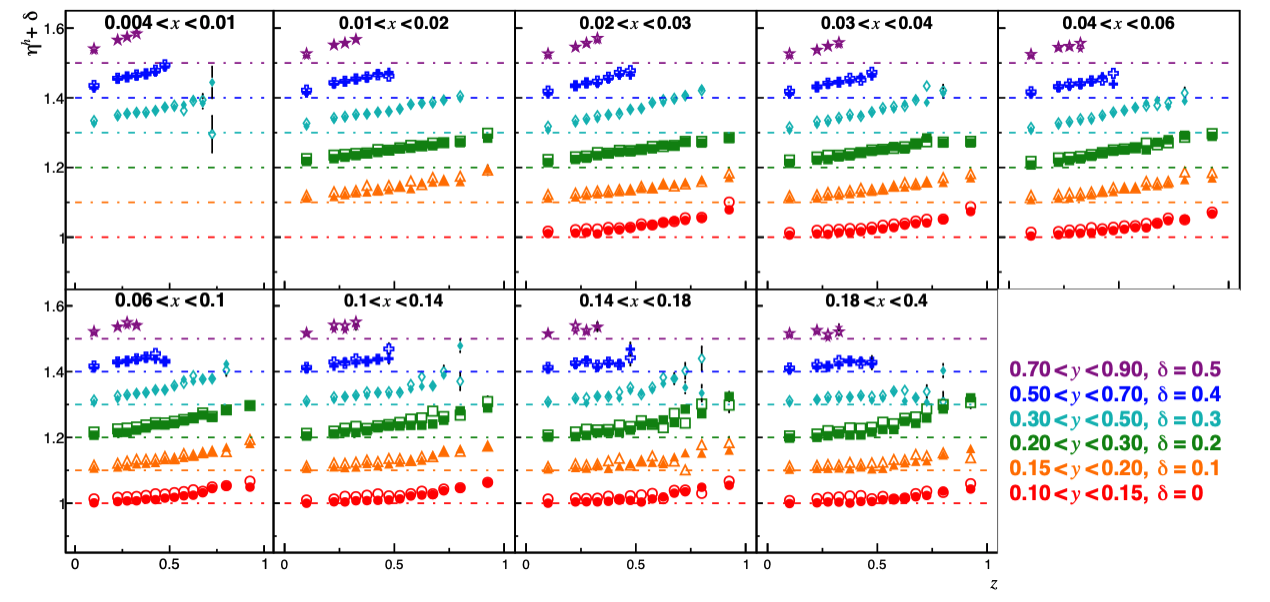
\includegraphics[scale=0.5]{./gfx/RadCor.png}
	\caption{Radiative correction factor $\eta^{h}$ for hadrons versus $z$ in bins of $x$ and staggered vertically with $y$. The full markers correspond to positive hadrons and open markers for negative hadrons.}
	\label{RadCor}
\end{sidewaysfigure}

\newpage

\section{Systematic Errors} \label{Sys}

\subsection{Errors associated to the RICH unfolding}

The first stage of pion identification is based on the likelihood ratios : $LH(\pi)/LH(2^{nd})$ and $LH(\pi)/LH(bg)$. These cuts are optimized to minimize the
pions misidentified as kaons. The systematic error associated to the selection of these cuts is performed varying the cuts around optimized values. Two sets of
cuts \textit{loose} and \textit{severe} were used (see Table \ref{loose.severe})

\begin{table}[!h]
	\centering
	\begin{tabular}{ccccccc}
		\hline
		 & \multicolumn{3}{c}{Loose} & \multicolumn{3}{c}{Severe} \\
		\hline
		 & $\pi$ & $K$ & $p(\bar{p})$ & $\pi$ & $K$ & $p(\bar{p})$ \\
		\hline
		$\frac{LH(\pi)}{LH(2^{nd})}$ & $> 1.00$ & $-$ & $-$ & $>1.06$ & $-$ & $-$ \\
		$\frac{LH(\pi)}{LH(bg)}$ & $> 2.00$ & $-$ & $<2.3$ $(2.2)$ & $>2.04$ & $-$ & $<2.0$ $(1.9)$ \\
		$\frac{LH(K)}{LH(2^{nd})}$ & $-$ & $>1.06$ & $-$ & $>-$ & $>1.10$ & $-$ \\
		$\frac{LH(K)}{LH(bg)}$ & $-$ & $>2.00$ & $<3.0$ $(2.9)$ & $-$ & $>2.16$ & $<2.7$ $(2.6)$ \\
		\hline
	\end{tabular}
  \caption{Set of loose and severe cuts to evaluate the RICH systematic errors.}
  \label{loose.severe}
\end{table}

To evaluate the systematic error associated to the selection of the particle likelihood cuts, the particle identification is performed using the \textit{loose}
and \textit{severe} sets of likelihood cuts and the corresponding RICH probability matrices and final multiplicities are extracted ($M^{h^{\pm},loose}_{raw}$
and $M^{h^{\pm},severe}_{raw}$ respectively). The largest difference between $M^{h^{\pm},loose}_{raw}$ and $M^{h^{\pm},severe}_{raw}$ with the nominal
multiplicity $M^{h^{\pm}}_{raw}$ is taken as an estimate of the systematic error :

\begin{equation}
  \sigma^{RICH_{LH}}_{sys} = MAX(|M^{h^{\pm},loose}_{raw}-M^{h^{\pm}}_{raw}|,|M^{h^{\pm},severe}_{raw}-M^{h^{\pm}}_{raw}|)
\end{equation}

The difference between the altered RICH probability matrices and the optimal one are plotted in Figs.\ref{Sysplus} and \ref{Sysminus}. For pions and protons, the largest differences
($<$5\%) are observed in the high momentum $p_h$ region. For kaons the difference reaches 4\% at low $p_h$ ; small differences ($<$1\%) are observed at the
highest $p_h$ value.

A second source of systematic error is that associated with the calculation of the RICH probability matrices. This is estimated by generating two sets of altered
RICH probability matrices. As represented in Eq.\ref{StatMat} the matrices are constructe using the statistical error associated to the original probability matrix elements.

\begin{figure}[!p]
	\centering
	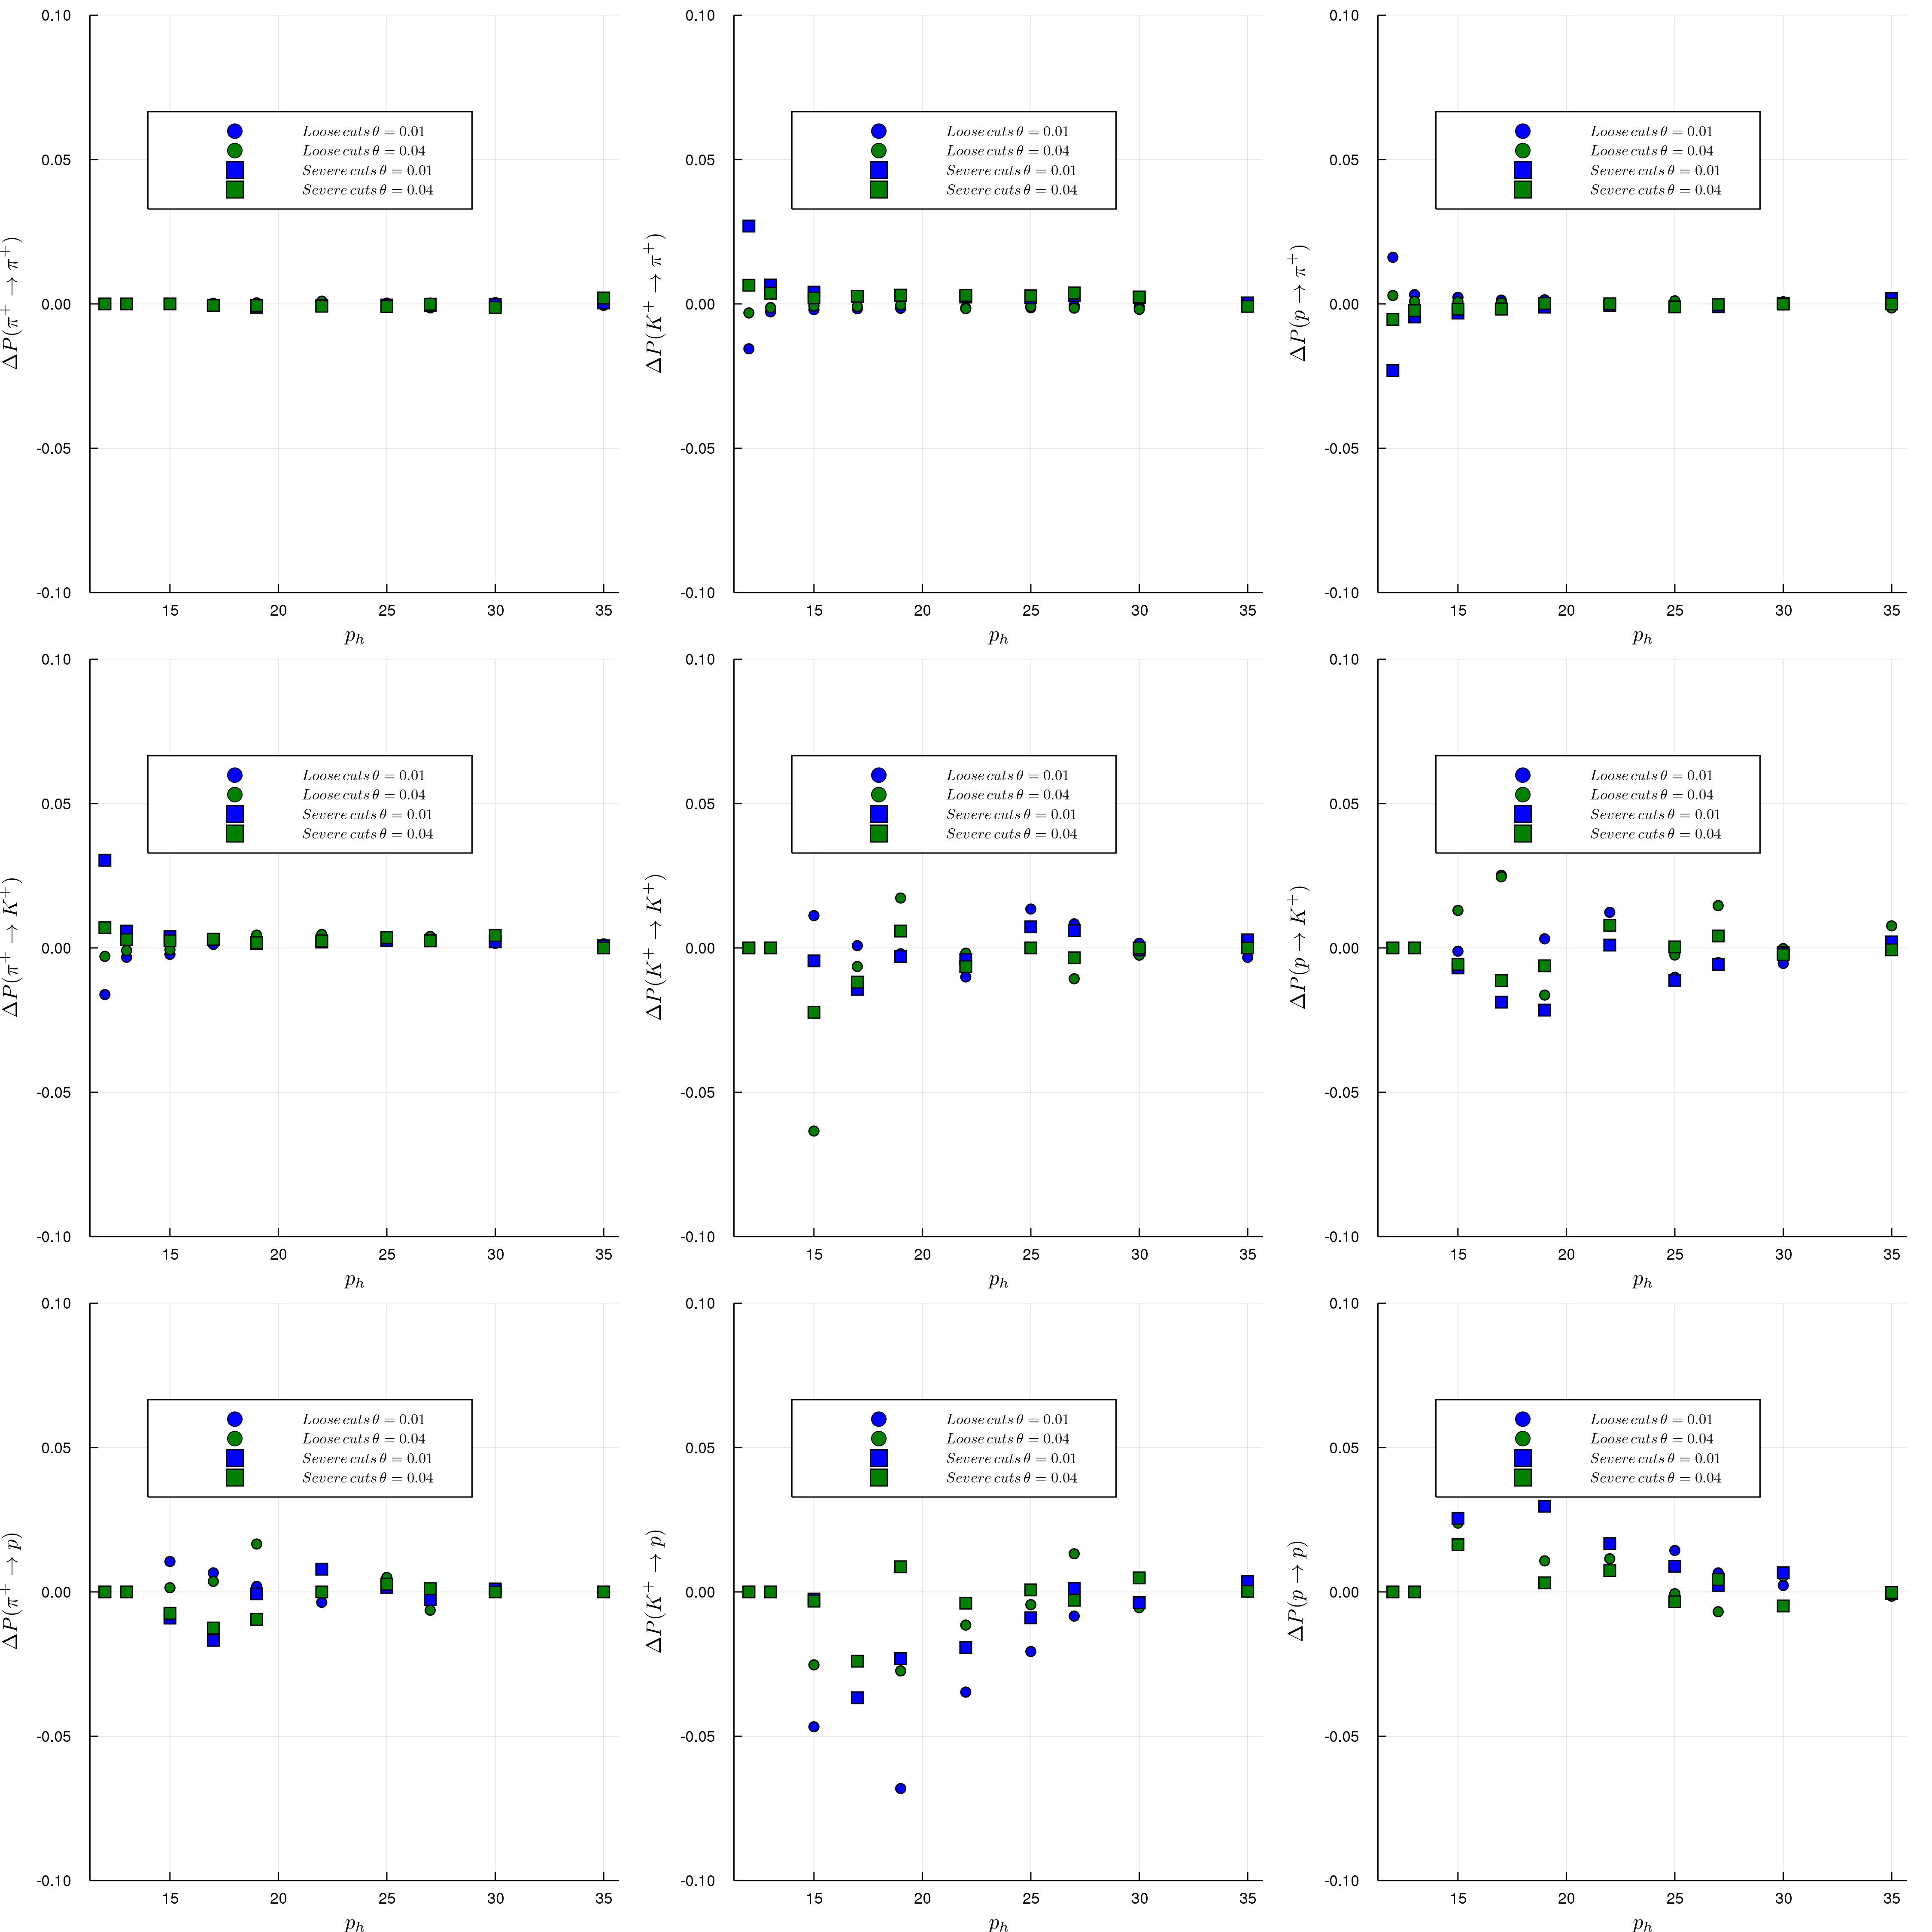
\includegraphics[scale=0.1]{./gfx/SysPlus.png}
	\caption{Difference between the identification and misidentification probabilities of loose and severe cuts with the optimal cuts for positive hadrons.}
	\label{Sysplus}
\end{figure}

\begin{figure}[!p]
	\centering
	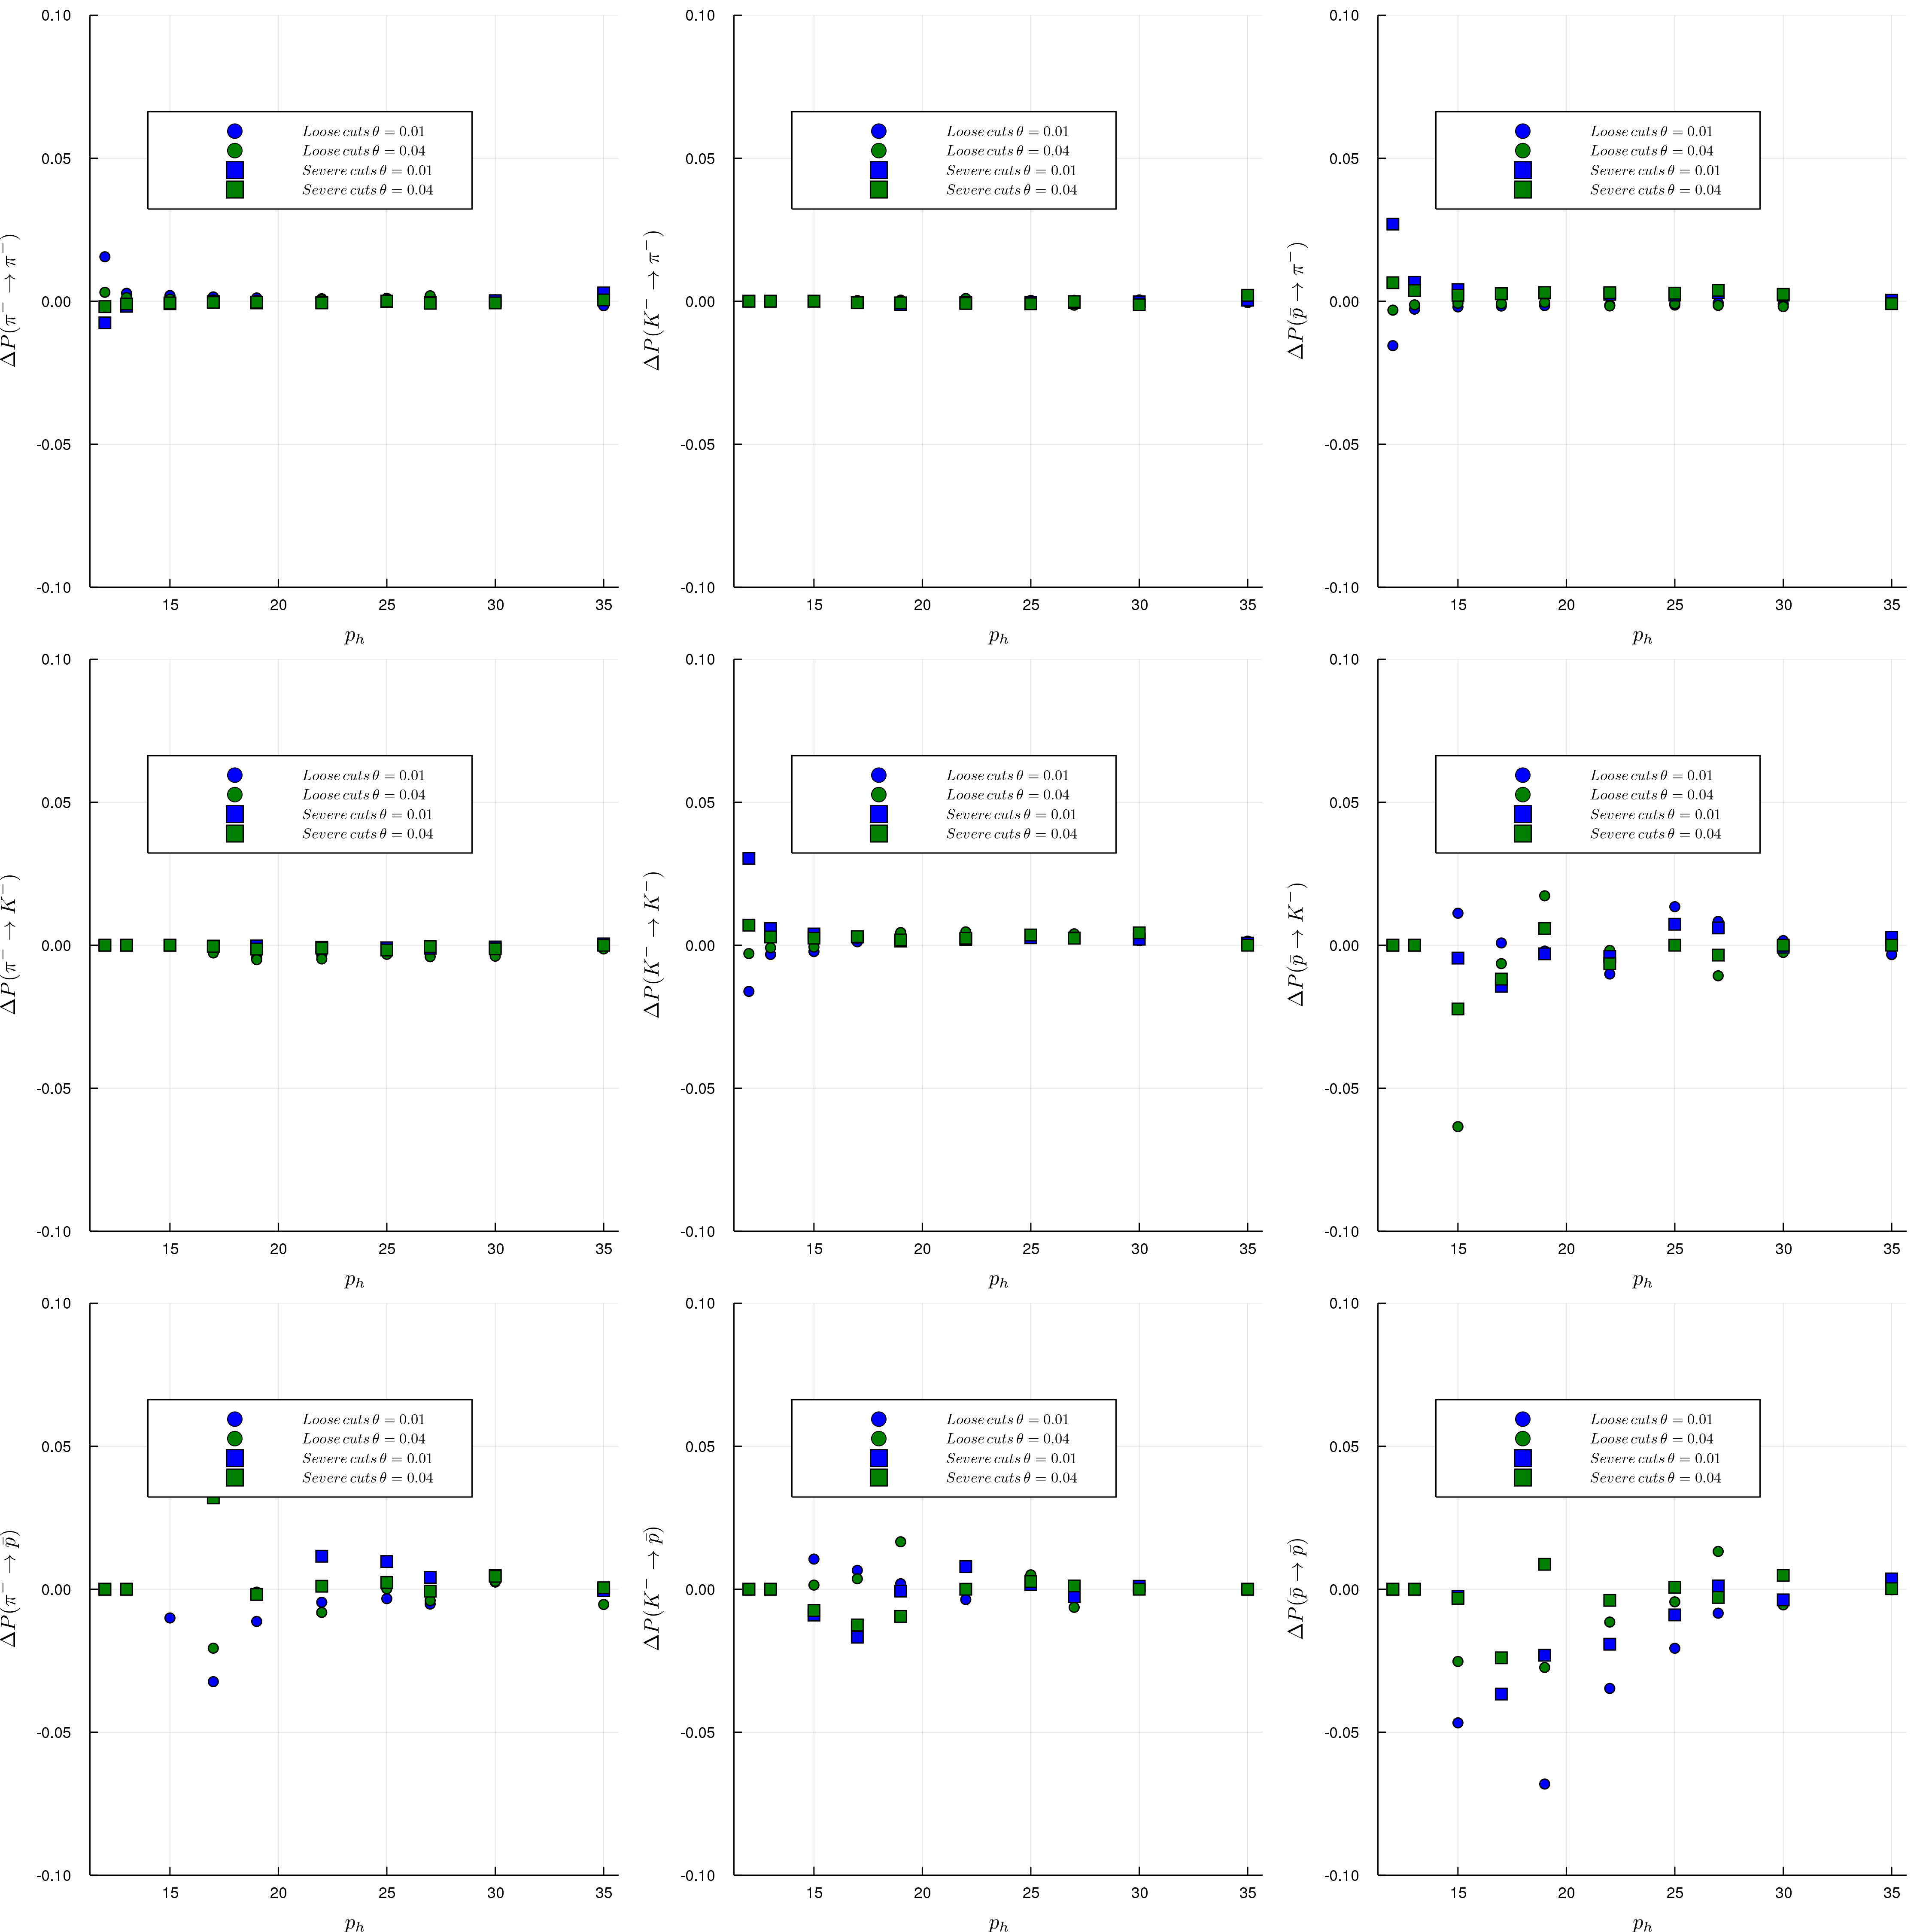
\includegraphics[scale=0.1]{./gfx/SysMinus.png}
	\caption{Difference between the identification and misidentification probabilities of loose and severe cuts with the optimal cuts for negative hadrons.}
	\label{Sysminus}
\end{figure}

\begin{equation}
  M^{\pm}_{RICH}
  =
  \begin{bmatrix}
  P(\pi \rightarrow \pi)\pm\sigma_{P(\pi \rightarrow \pi)} & P(K \rightarrow \pi)\mp\sigma_{P(K \rightarrow \pi)} & P(p \rightarrow \pi)\mp\sigma_{P(p \rightarrow \pi)}\\
  P(\pi \rightarrow K)\mp\sigma_{P(\pi \rightarrow K)} & P(K \rightarrow K)\pm\sigma_{P(K \rightarrow K)} & P(p \rightarrow K)\mp\sigma_{P(p \rightarrow K)} \\
  P(\pi \rightarrow p)\mp\sigma_{P(\pi \rightarrow p)} & P(K \rightarrow p)\mp\sigma_{P(K \rightarrow p)} & P(p \rightarrow p)\pm\sigma_{P(p \rightarrow p)}
  \end{bmatrix}
	\label{StatMat}
\end{equation}

The raw multiplicities $M^{h^{\pm},+}_{raw}$ and $M^{h^{\pm},-}_{raw}$ are then recalculated using the altered probability matrices. The largest difference between
$M^{h^{\pm},+}_{raw}$ and $M^{h^{\pm},-}_{raw}$ with $M^{h^{\pm}}_{raw}$ is taken as the sytematic error :

\begin{equation}
  \sigma^{RICH_{stat}}_{sys} = MAX(|M^{h^{\pm},+}_{raw}-M^{h^{\pm}}_{raw}|,|M^{h^{\pm},-}_{raw}-M^{h^{\pm}}_{raw}|)
\end{equation}

The final systematic uncertainty associated to the particle identification and unfolding correction ($\sigma^{RICH}_{sys}$) is the largest value of $\sigma^{RICH_{stat}}_{sys}$ and $\sigma^{RICH_{LH}}_{sys}$. The error goes from $<$ 0.2\% at low $y$ for all $x$ and $z$ bins to $\sim$ 20\% for high $y$ and high $z$, where multiplicities are low.



\subsection{Errors associated to acceptance (z-vertex dependence)}

The correction of extracted multiplicities for limited geometric acceptance of the apparatus and the detector resolution is estimated using a Monte-Carlo simulation as described in Section \ref{Cor}. This correction should be independant of the model used in the MC simulation. For this reason, the acceptance estimation has been evaluated using different MC samples, obtainined by changing the quark fragmentation parameters from JETSET and by using different parton distribution functions in LEPTO. This exercise has been performed in a previous release \cite{Release2015} and a conservative systematic error of $\sim$ 5\% was derived.
Another error concerns the z-vertex dependence : the target can be separated into 4 different parts and the sum of multiplicities extracted from each part is then compared. From this comparison, a conservative systematic error of $\sim$ 5\% was derived.
These values are taken provisionally for the estimation shown in Section \ref{Res}.

\subsection{Stability over time}

The data samples used in the analysis were recorded over a period of 5 weeks. As a quality check, the sum and ratio of multiplicities in the different weeks were compared to the sum and ratio of multiplicities over the overall 5 weeks of data and the multiplicities averaged over y were compared period by period. The compatibility between weeks was found to be below the 1\% level within statistical fluctuations. Consequently, no systematic error will be assigned for the data compatibility.

\subsection{Stability over beam charge}

The data samples used in the analysis were recorded with two different beam charge. As a quality check, the multiplicities averaged over y were compared for both beam charge. The compatibility between the two beam charge was found to be below the 1\% level within statistical fluctuations. Consequently, no systematic error will be assigned for the beam charge change.

\subsection{Error associated to the diffractive vector meson correction}

In HEPGEN, the cross section for exclusive vector meson production is normalized to the GPD model of Goloskokov and Kroll. The theoretical uncertainty on the predicted cross section close to COMPASS kinematics is around 30\% \cite{Goloskokov}. Propagating this uncertainty leads to a maximum relative uncertainty under 6\%.
The method for the correction of nuclear effects maily changes the shape of the $p_T^2$ distribution with respect to the diffractive vector meson production on a free nucleon. It assumes that the $p_T^2$-integrated nuclear cross-section per nucleon for exclusive events is the same as the $p_T^2$-integrated nuclear cross section for a free nucleon. According to A. Sandacz \cite{Hepgen}, the systematic uncertainty due to this assumption is a few percent.

\section{Results} \label{Res}

For the final multiplicities, it yields :

\begin{equation}
	M_{Final}(x,y,z) = \frac{M_{raw}(x,y,z)}{A(x,y,z)}B(x,y,z)
\end{equation}

\subsection{3-dimensional binning in x, y and z}

The final multiplicities with all corrections are shown in a multidimensional binning in $x$, $y$ and $z$ (9 columns, 5 rows and 12 points) in Figs. \ref{hp}, \ref{hm}, \ref{Pip}, \ref{Pim}, \ref{pp}, \ref{pm}, \ref{Kp} and \ref{Km}. Bins with acceptance $<$ 30\% and those whose $<y>$ is less than 6\% of the binwidth to the bin edge with poor statistics ($\sigma$ $>$ 0.02) have been excluded and are not shown. The latter exclusion is applied to remove bins that lie on the edge of the kinematic acceptance region. The band shown at the bottom of each plot correspond to the systematic error. The statistical uncertainties are shown, however they are mostly smaller than the size of the points.

\begin{sidewaysfigure}[!p]
	\centering
	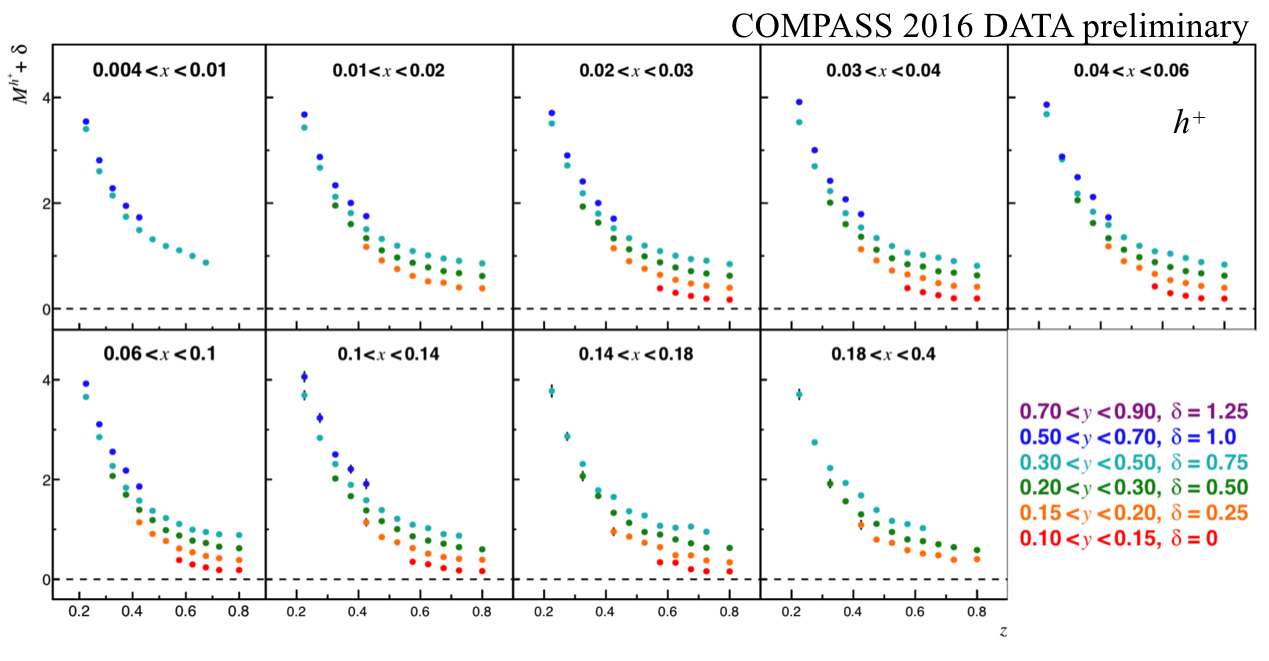
\includegraphics[scale=0.5]{./gfx/hp.png}
	\caption{Final positive hadron multiplicities as a function of $z$ in bins of $x$ and staggered vertically with $y$. Radiative correction, diffractive vector meson correction and acceptance correction have been applied. All systematic errors are shown in band for the bin 0.3 $< y <$ 0.5.}
	\label{hp}
\end{sidewaysfigure}

\begin{sidewaysfigure}[!p]
	\centering
	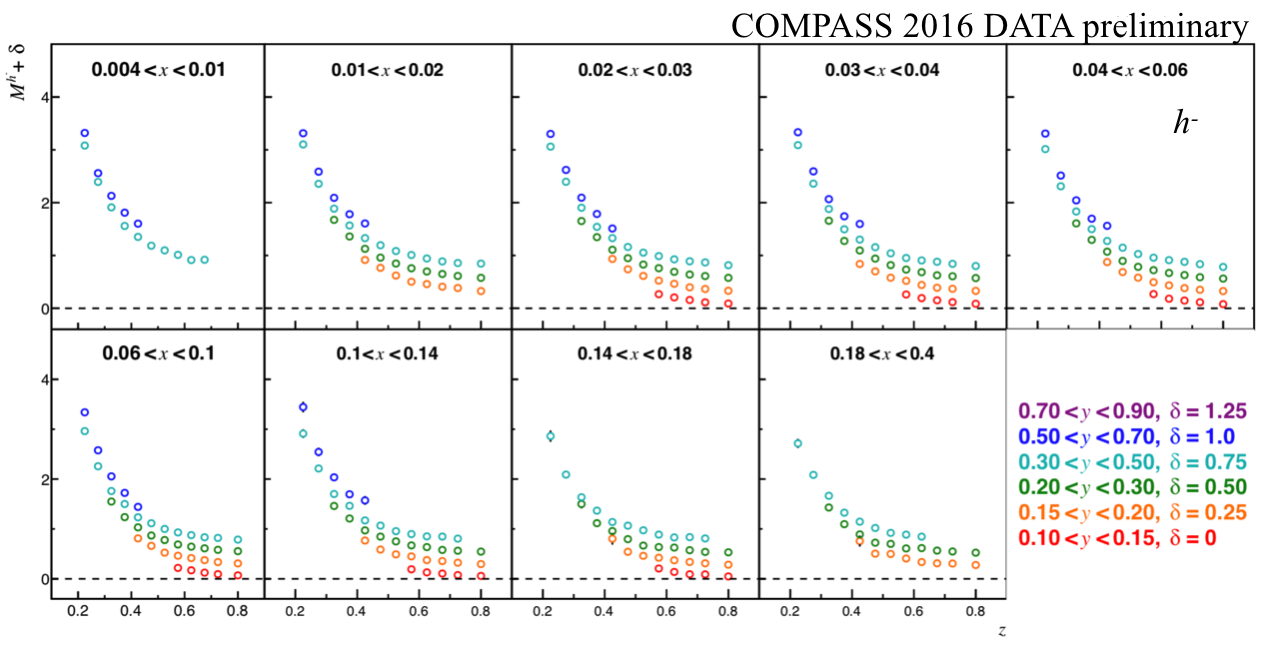
\includegraphics[scale=0.5]{./gfx/hm.png}
	\caption{Final negative hadron multiplicities as a function of $z$ in bins of $x$ and staggered vertically with $y$. Radiative correction, diffractive vector meson correction and acceptance correction have been applied. All systematic errors are shown in band for the bin 0.3 $< y <$ 0.5.}
	\label{hm}
\end{sidewaysfigure}

\begin{sidewaysfigure}[!p]
	\centering
	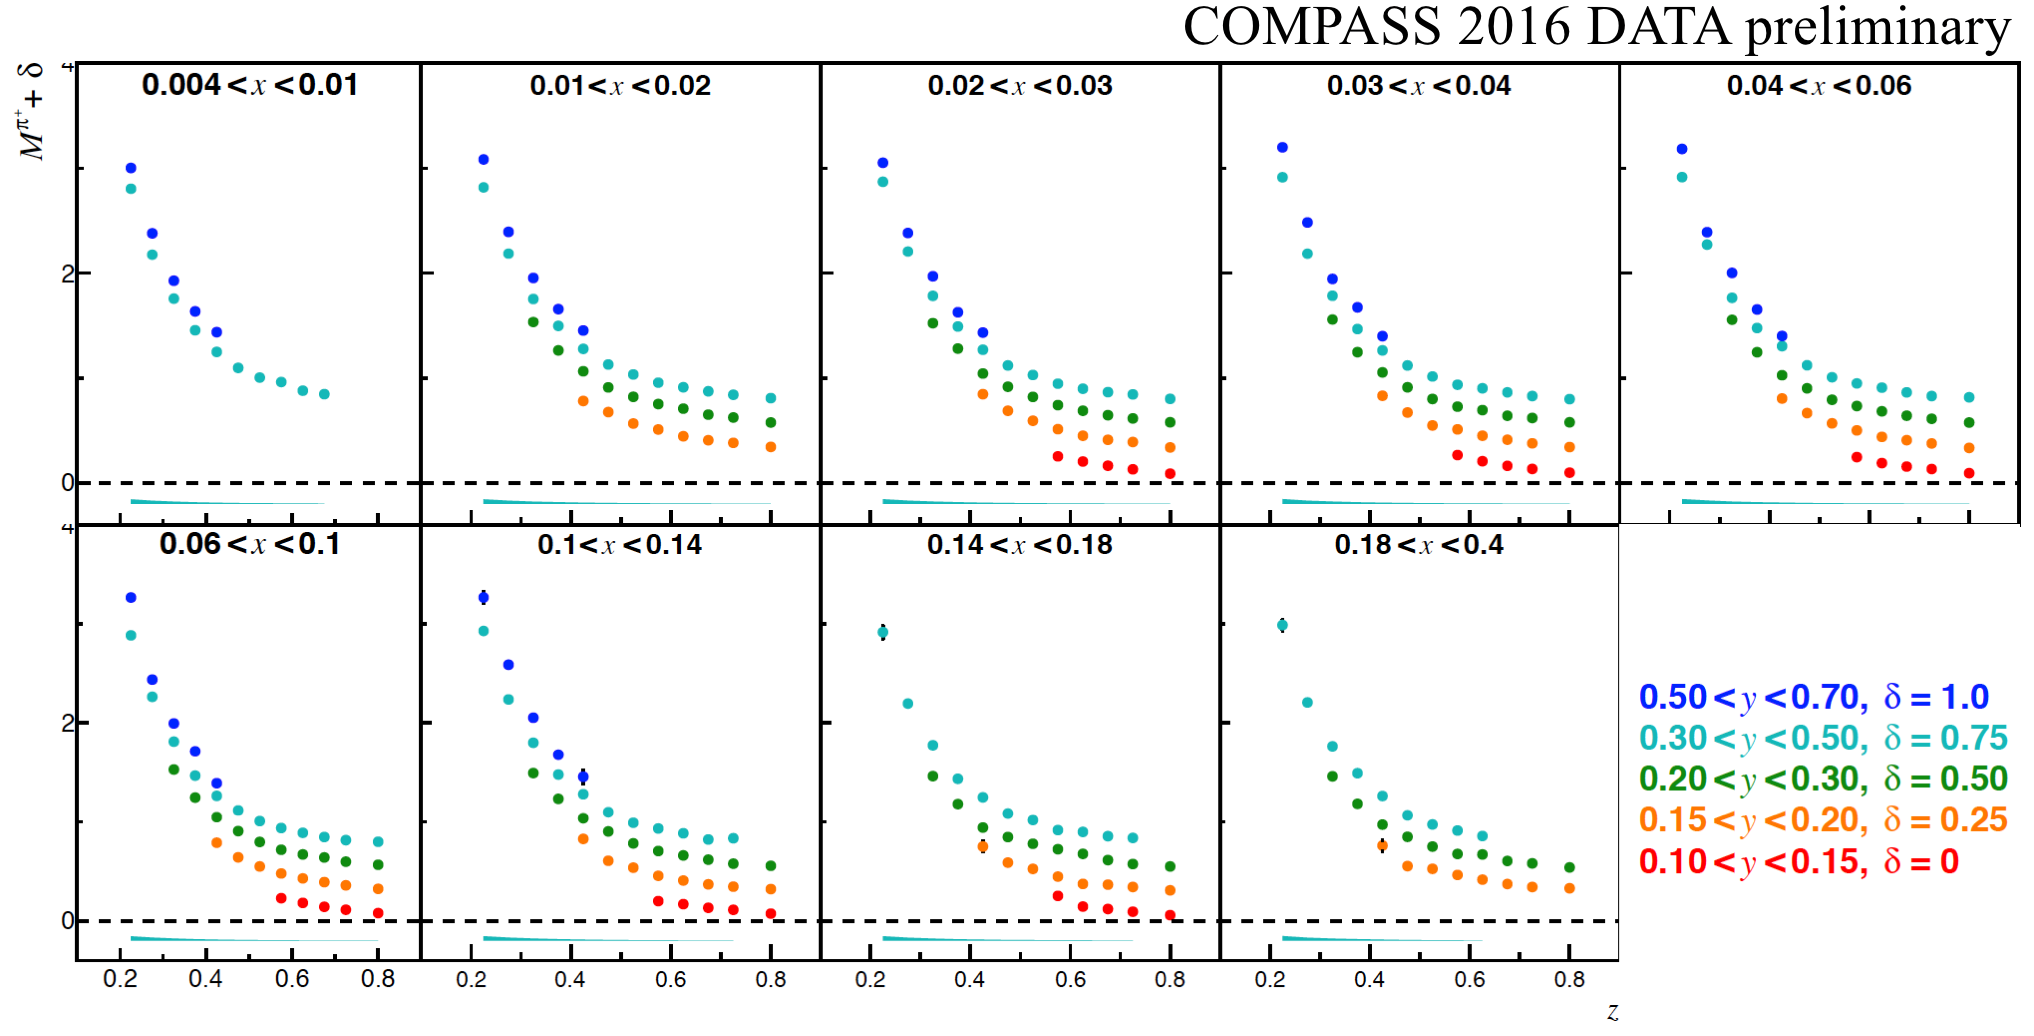
\includegraphics[scale=0.5]{./gfx/Pip.png}
	\caption{Final positive pion multiplicities as a function of $z$ in bins of $x$ and staggered vertically with $y$. Radiative correction, diffractive vector meson correction and acceptance correction have been applied. All systematic errors are shown in band for the bin 0.3 $< y <$ 0.5.}
	\label{Pip}
\end{sidewaysfigure}

\begin{sidewaysfigure}[!p]
	\centering
	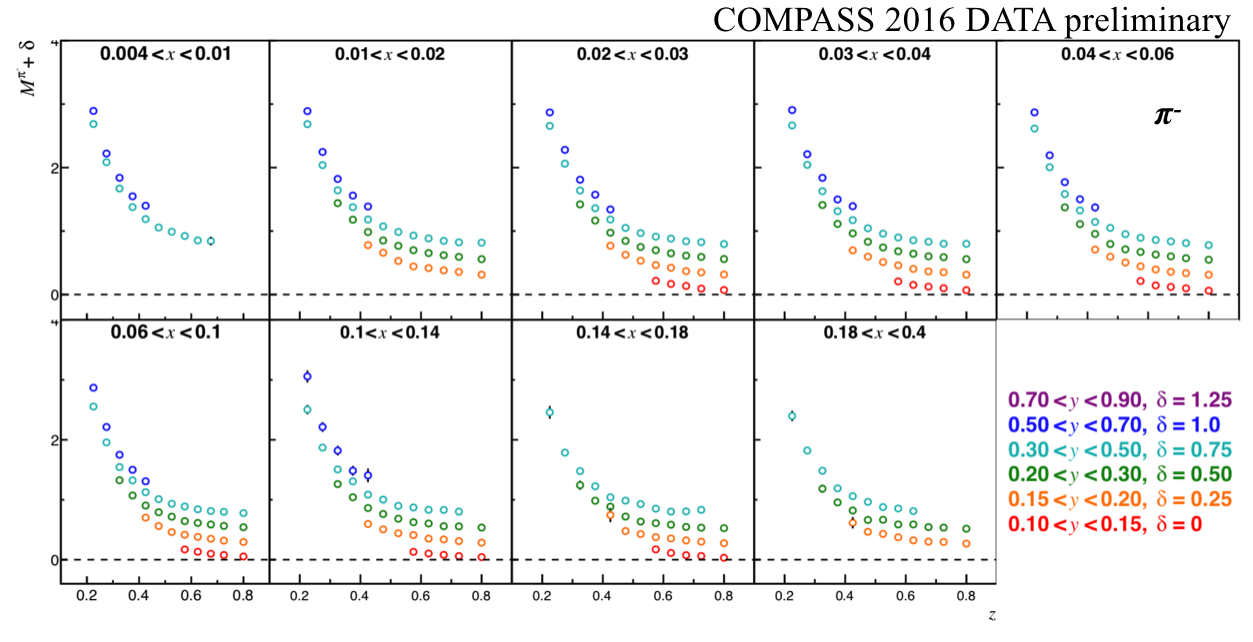
\includegraphics[scale=0.5]{./gfx/Pim.png}
	\caption{Final positive pion multiplicities as a function of $z$ in bins of $x$ and staggered vertically with $y$. Radiative correction, diffractive vector meson correction and acceptance correction have been applied. All systematic errors are shown in band for the bin 0.3 $< y <$ 0.5.}
	\label{Pim}
\end{sidewaysfigure}

\begin{sidewaysfigure}[!p]
	\centering
	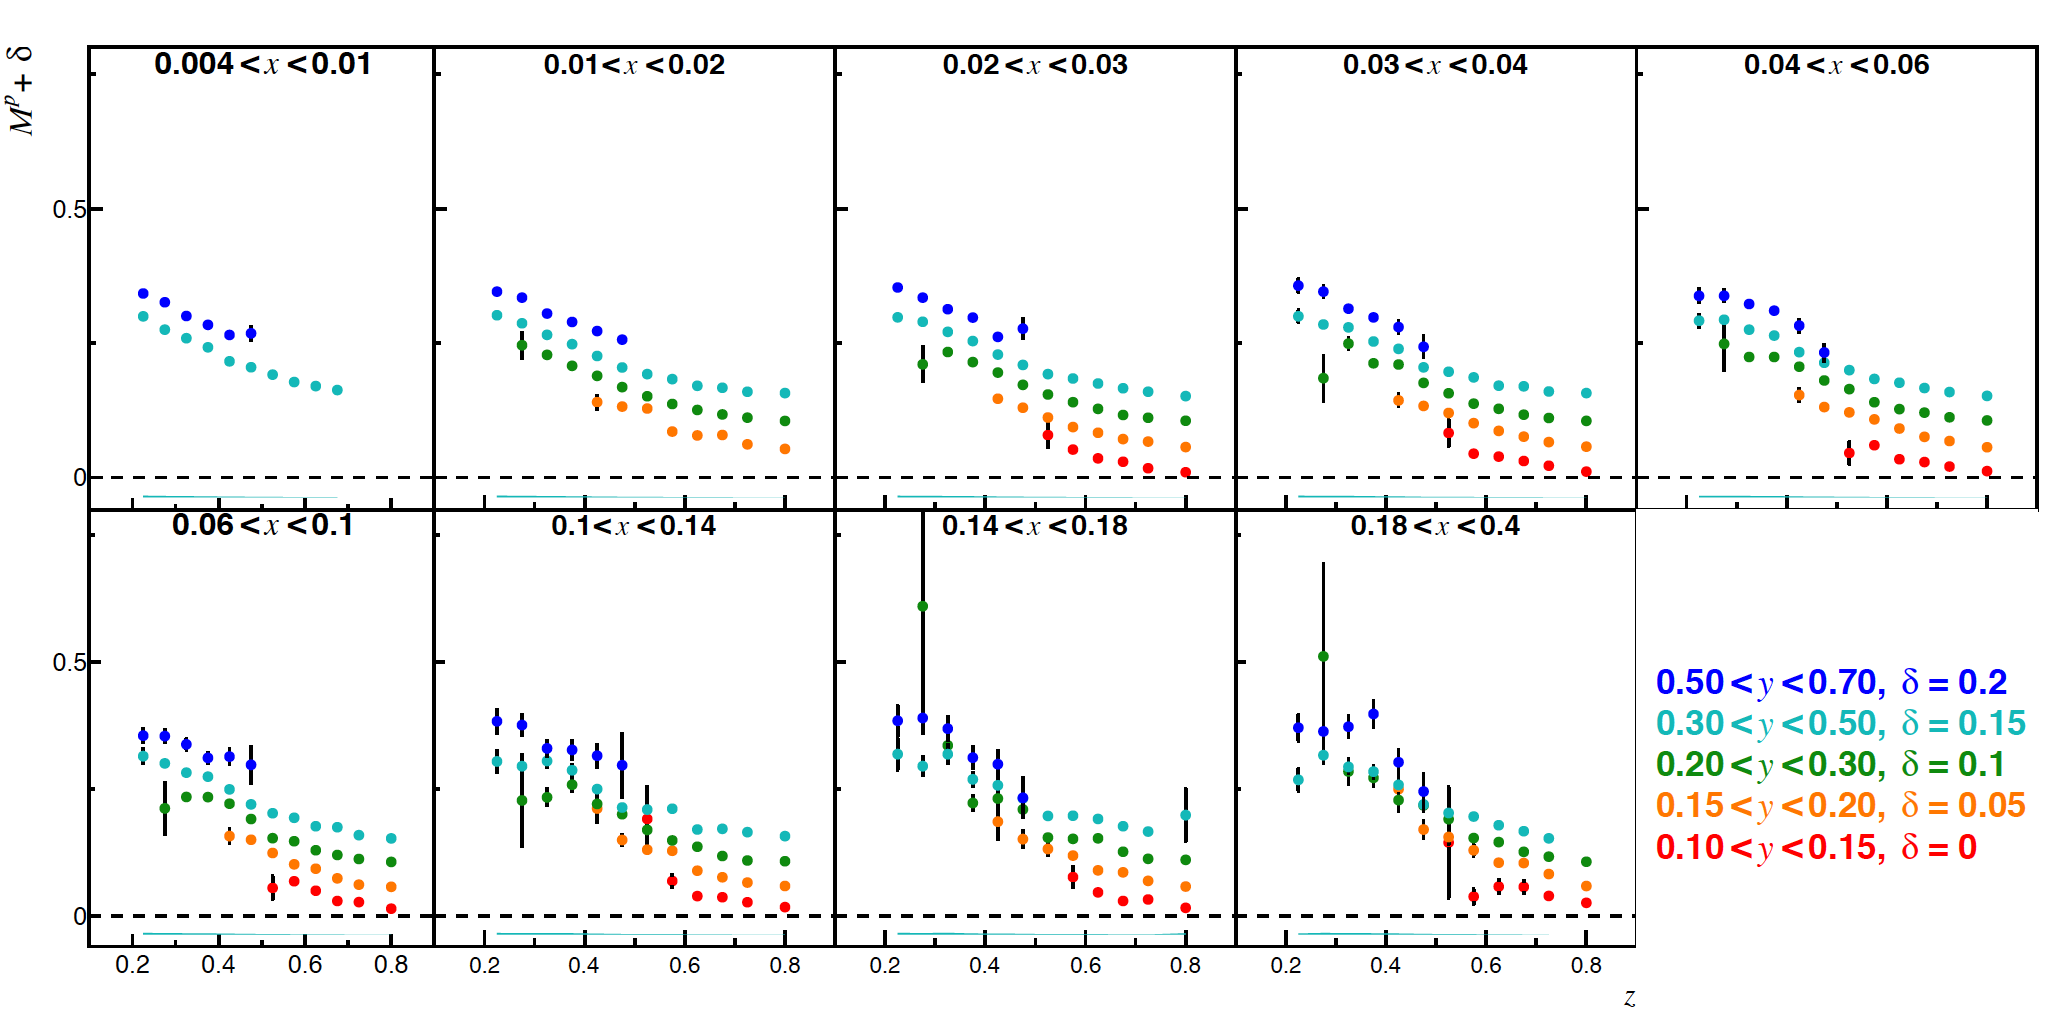
\includegraphics[scale=0.5]{./gfx/pp.png}
	\caption{Final positive proton multiplicities as a function of $z$ in bins of $x$ and staggered vertically with $y$. Radiative correction, diffractive vector meson correction and acceptance correction have been applied. All systematic errors are shown in band for the bin 0.3 $< y <$ 0.5.}
	\label{pp}
\end{sidewaysfigure}

\begin{sidewaysfigure}[!p]
	\centering
	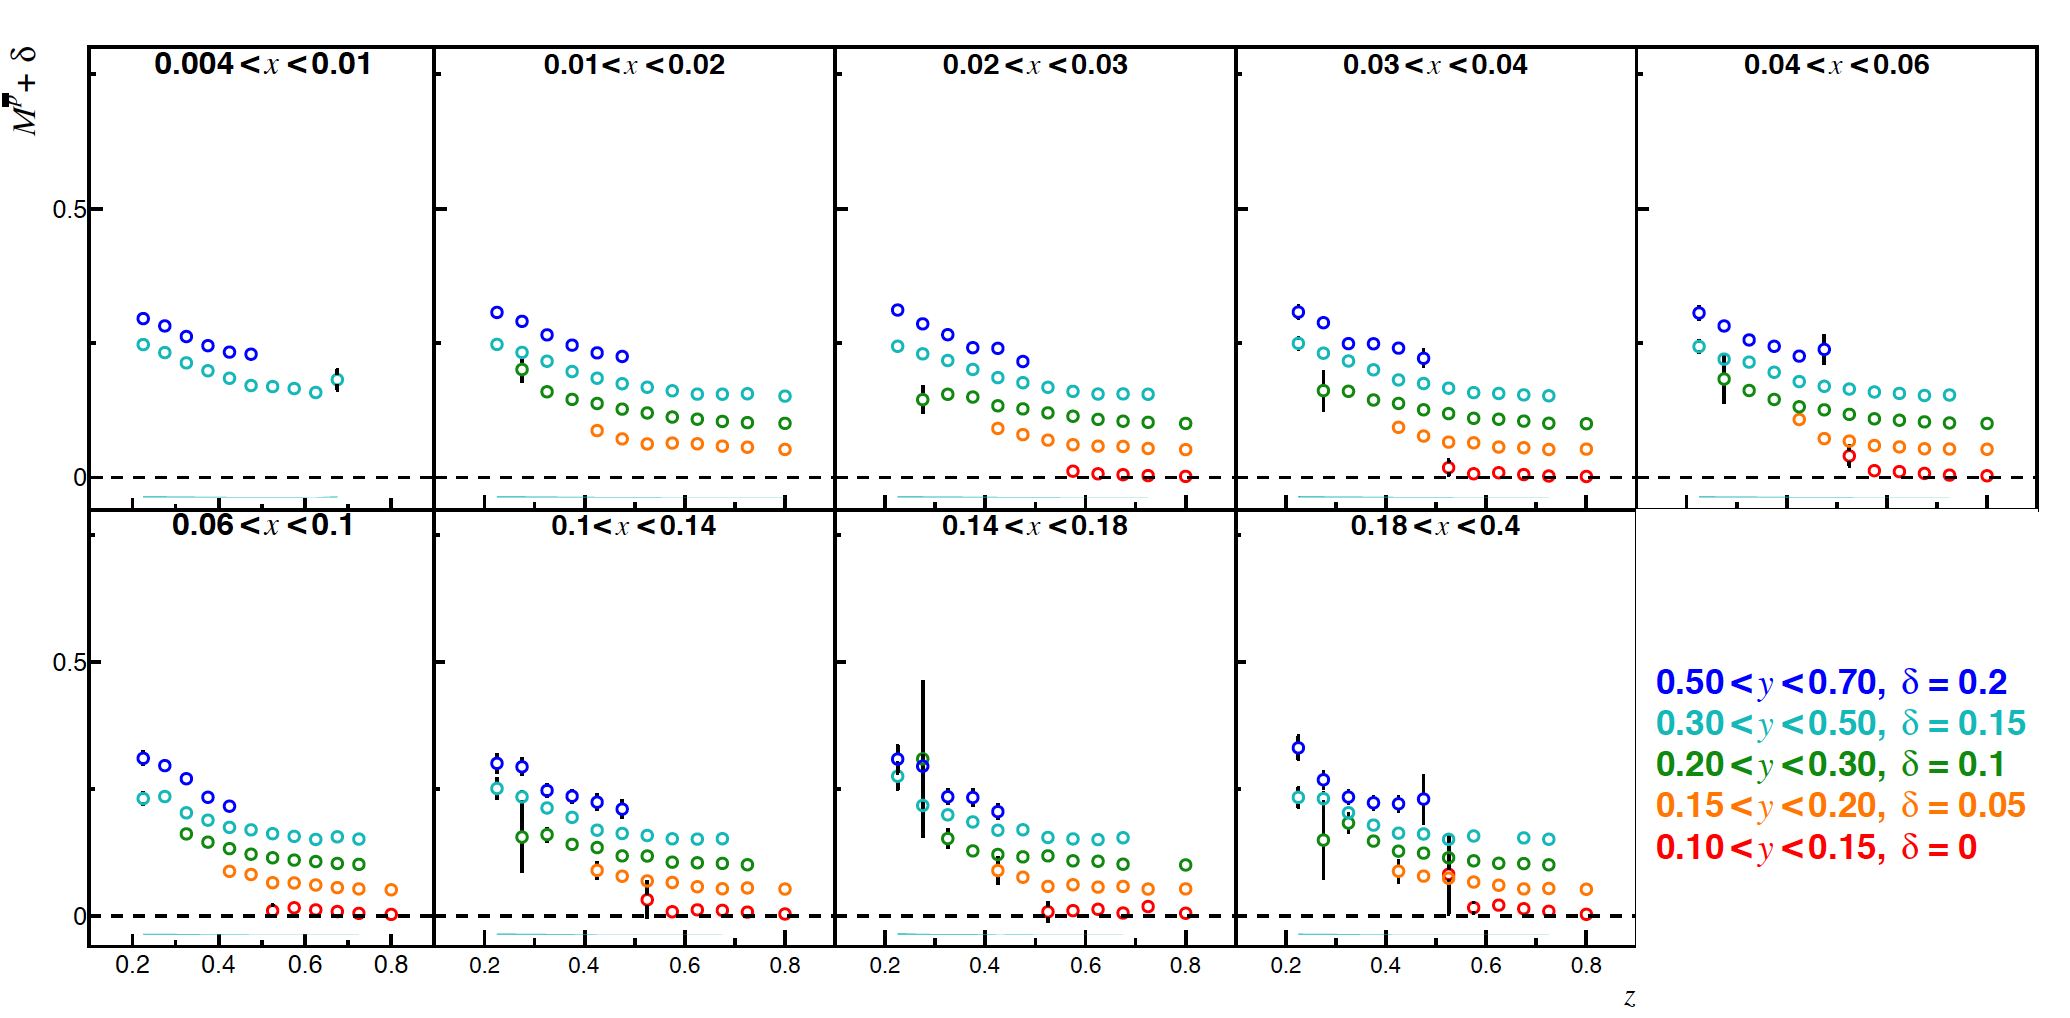
\includegraphics[scale=0.5]{./gfx/pm.png}
	\caption{Final positive proton multiplicities as a function of $z$ in bins of $x$ and staggered vertically with $y$. Radiative correction, diffractive vector meson correction and acceptance correction have been applied. All systematic errors are shown in band for the bin 0.3 $< y <$ 0.5.}
	\label{pm}
\end{sidewaysfigure}

\newpage

\section{Sum and ratio of charged hadrons multiplicities $M^{h^+}$ and $M^{h^-}$} \label{MSR}

One of the main goal of the multiplicity analysis is the extraction of kaon strange quark fragmentation functions. These fragmentation functions allow us to extract the strange quark polarization in the nucleon obtained from SIDIS analyses. From this point of view the sum of positive and negative kaon hadrons multiplicities over $z$ is of special interest.

The actual results are presented in Figs. \ref{hs} to \ref{Kr}. The data are integrated over $z$ (0.2 to 0.85) and averaged over $y$ (0.1 to 0.7). Only the 8 $x$ bins that have a sufficient $z$ coverage subsist.
All the sum and ratio are compared with their isoscalar counterpart from our publication of charged hadrons, pions and kaons on isoscalar target and also with HERMES results obtained on proton and deuteron.

All the 2016 results for the sum seem to suffer from a drop a high $x$, particularly visible on hadrons and pions. The kaons seem to be less harmed by this issue. The cause of this drop is still under investigation and might probably be caused by a bad tuning of some hadron variables like $\theta_h$. In 2006 analysis, the high-$p_T$ tuning of the Monte-Carlo simulation was giving solid description for this variable when in 2016 analysis, with the same tuning, there is a great discrepancy between data and Monte-Carlo that might play a role in the aforementionned issue.

The hadron sum for proton target should lie at the same level than our isoscalar results. The discrepancy in amplitude can be explained by the fact that our radiative correction at the time of the publication were not correct and with our nowadays knowledge of radiative corrections, we know that we should move up all the points by $\sim$6\%, which reconcile proton and isoscalar results within error bars. The same reasoning can be made for the pion sum.

The kaon sum for proton target should be slightly ($\sim$5-10\%) above our isoscalar results. For the isoscalar results for kaons, contrary to hadrons and pions, an additional $5\%$ was added to the results to take into account the bad knowledge of the radiative correction at the time. The discrepancy with HERMES results, already seen in the isoscalar case, remains.

The hadron and pion ratio on proton target should lie above our isoscalar results, the reason being the different quark mixture in the two targets (more $u$ in proton target thus higher $\pi+$/$\pi-$ ratio in proton than in isoscalar). The difference is expected to be $\sim$10-20\%. For the very same reason, the kaon ratio on proton target is expected to be bigger than our isoscalar result by $\sim$10\%.

As the kaon results are the less affected by the high $x$ drop and also are the most interesting for the community, we ask only the release of kaon related results. The hadron and pion results are too much sensitive at the moment due to this high $x$ problem, thus we do not want to ask a release for them yet.

\newpage

\begin{figure}[H]
	\centering
	\includegraphics[scale=0.55]{./gfx/hs.png}
	\caption{$\mathscr{M}^{h^+}+\mathscr{M}^{h^-}$ versus $x$ for \textit{COMPASS} data (proton in blue and isoscalar in red, closed points) averaged over $y$ (0.1 to 0.7) and integrated over $z$ (0.2 to 0.85). All systematic errors are shown point to point as a band.}
	\label{hs}
\end{figure}

\begin{figure}[H]
	\centering
	\includegraphics[scale=0.55]{./gfx/hr.png}
	\caption{$\mathscr{M}^{h^+}/\mathscr{M}^{h^-}$ versus $x$ for \textit{COMPASS} data (proton in blue and isoscalar in red, closed points) averaged over $y$ (0.1 to 0.7) and integrated over $z$ (0.2 to 0.85). All systematic errors are shown point to point as a band.}
	\label{hr}
\end{figure}

\newpage

\begin{figure}[H]
	\centering
	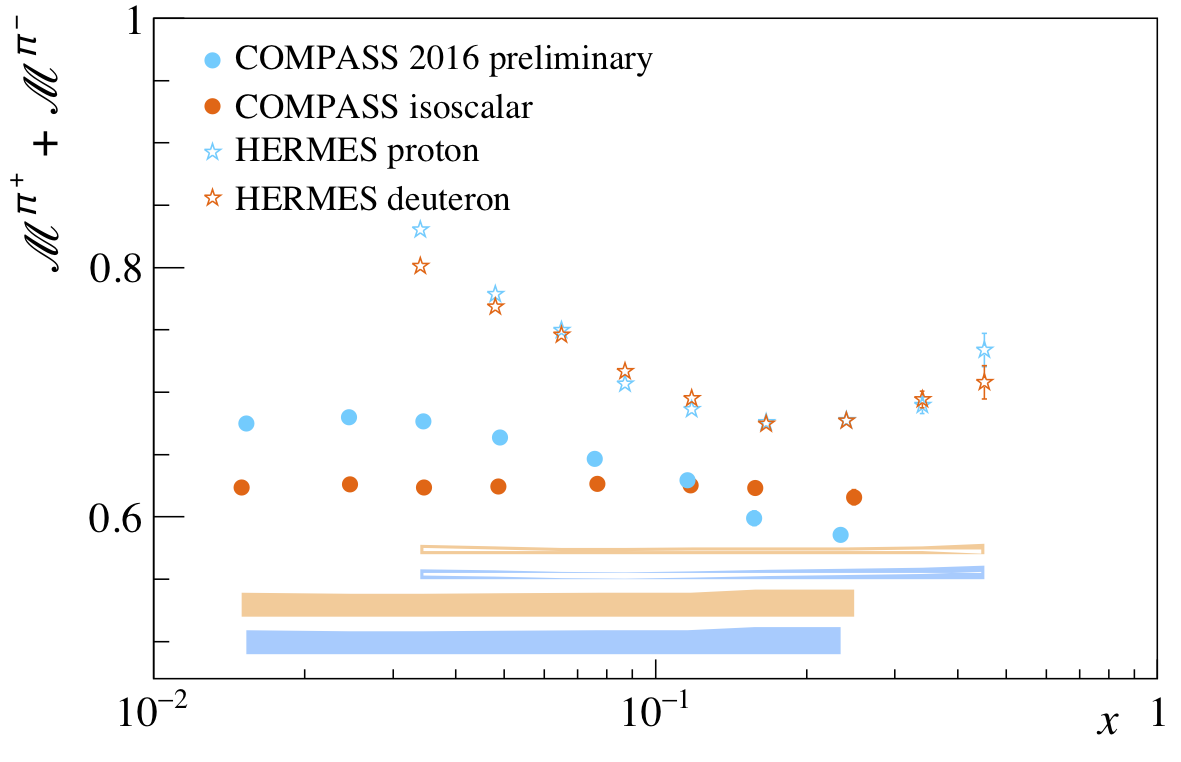
\includegraphics[scale=0.55]{./gfx/Pis.png}
	\caption{$\mathscr{M}^{\pi^+}+\mathscr{M}^{\pi^-}$ versus $x$ for \textit{COMPASS} data (proton in blue and isoscalar in red, closed points) averaged over $y$ (0.1 to 0.7) and integrated over $z$ (0.2 to 0.85) and \textit{HERMES} data \cite{HERMES} (proton in blue and deuteron in red, open points) averaged over $y$ (0.1 to 0.85) and integrated over $z$ (0.2 to 0.8). All systematic errors are shown point to point as a band.}
	\label{Pis}
\end{figure}

\begin{figure}[H]
	\centering
	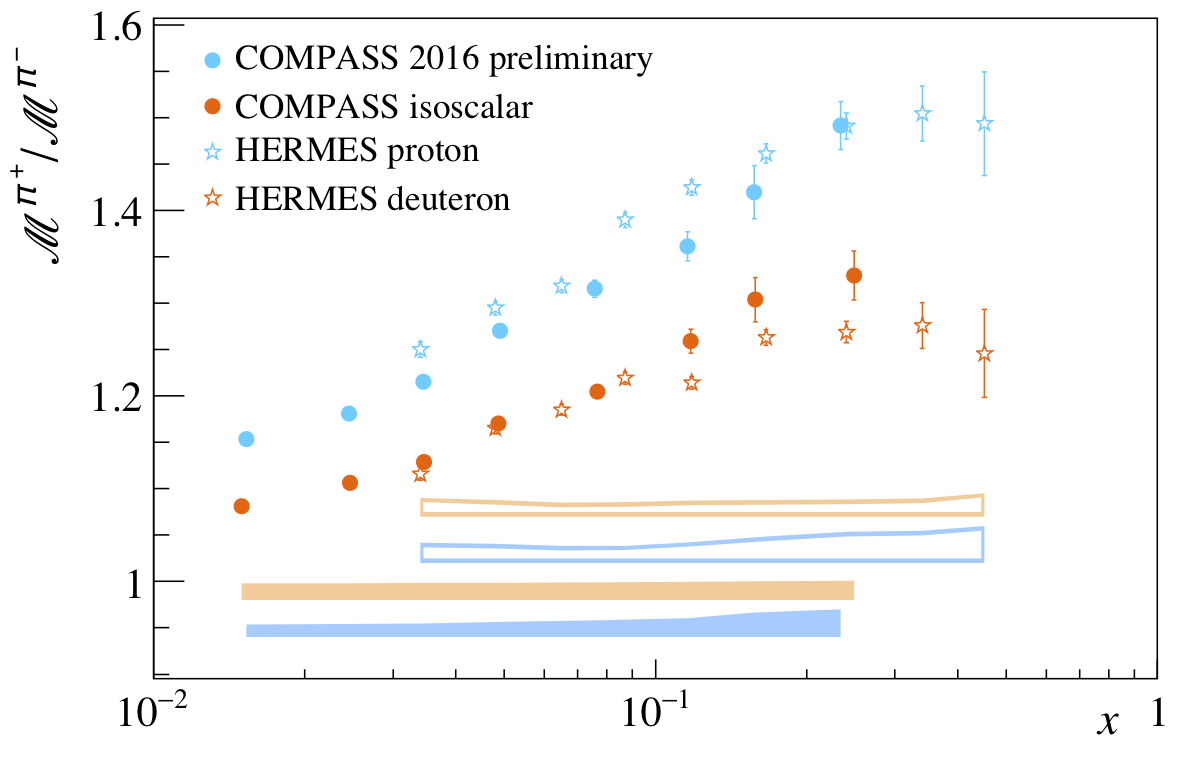
\includegraphics[scale=0.55]{./gfx/Pir.png}
	\caption{$\mathscr{M}^{\pi^+}/\mathscr{M}^{\pi^-}$ versus $x$ for \textit{COMPASS} data (proton in blue and isoscalar in red, closed points) averaged over $y$ (0.1 to 0.7) and integrated over $z$ (0.2 to 0.85) and \textit{HERMES} data \cite{HERMES} (proton in blue and deuteron in red, open points) averaged over $y$ (0.1 to 0.85) and integrated over $z$ (0.2 to 0.8). All systematic errors are shown point to point as a band.}
	\label{Pir}
\end{figure}

\begin{figure}[H]
	\centering
	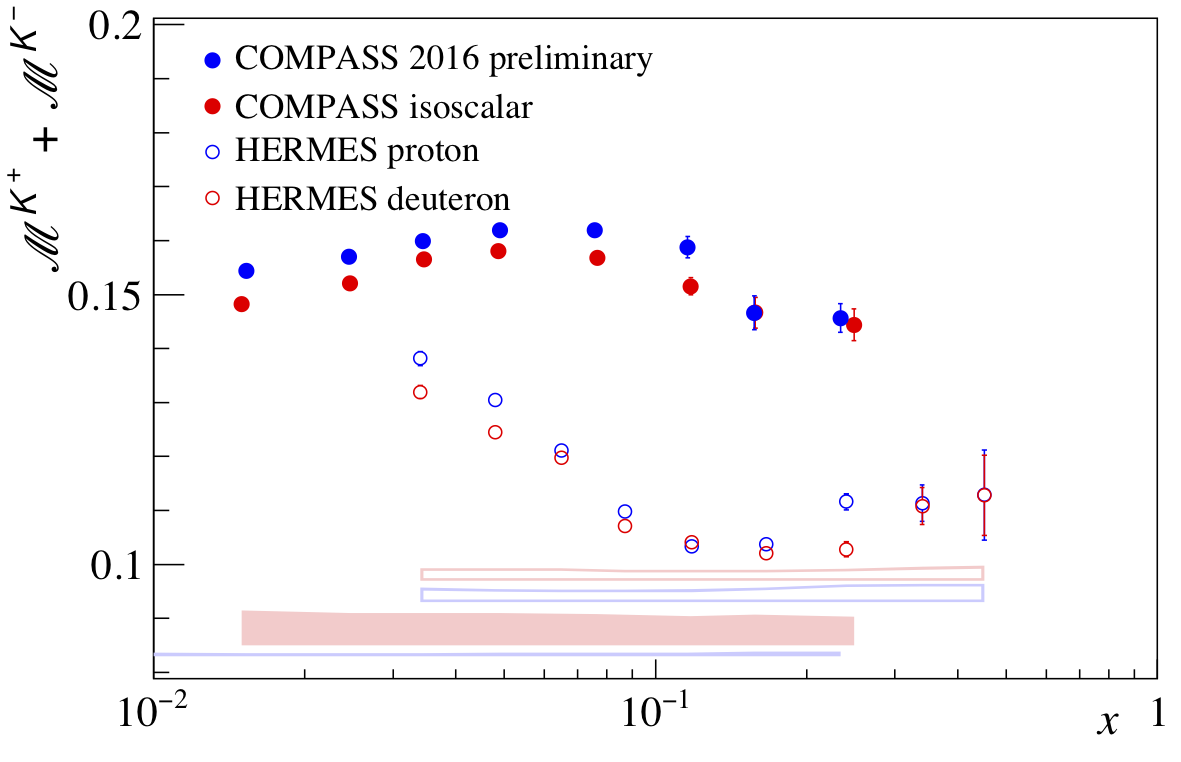
\includegraphics[scale=0.55]{./gfx/Ks.png}
	\caption{$\mathscr{M}^{K^+}+\mathscr{M}^{K^-}$ versus $x$ for \textit{COMPASS} data (proton in blue and isoscalar in red, closed points) averaged over $y$ (0.1 to 0.7) and integrated over $z$ (0.2 to 0.85) and \textit{HERMES} data \cite{HERMES} (proton in blue and deuteron in red, open points) averaged over $y$ (0.1 to 0.85) and integrated over $z$ (0.2 to 0.8). All systematic errors, including the asymmetric systematic errors for radiative correction for \textit{COMPASS} isoscalar kaons (100\% error, determined by removing the hadronic radiative corrections), are shown point to point as a band.}
	\label{Ks}
\end{figure}

\begin{figure}[H]
	\centering
	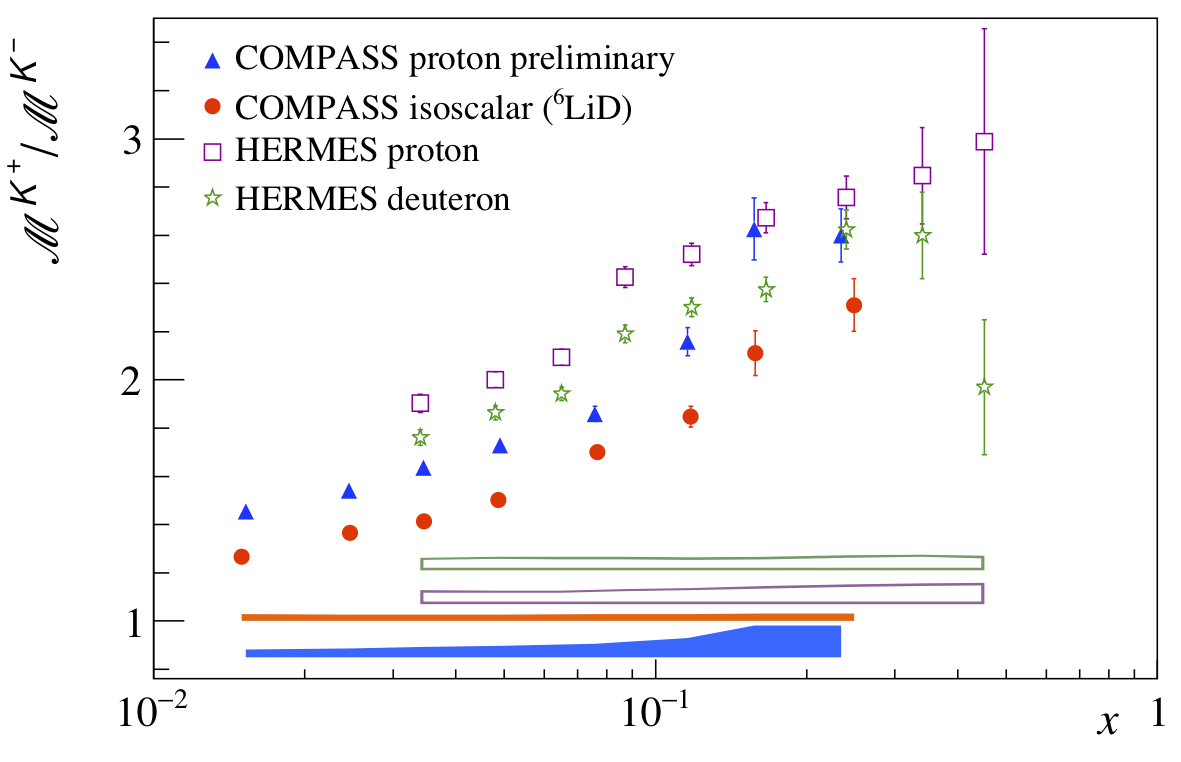
\includegraphics[scale=0.55]{./gfx/Kr.png}
	\caption{$\mathscr{M}^{K^+}/\mathscr{M}^{K^-}$ versus $x$ for \textit{COMPASS} data (proton in blue and isoscalar in red, closed points) averaged over $y$ (0.1 to 0.7) and integrated over $z$ (0.2 to 0.85) and \textit{HERMES} data \cite{HERMES} (proton in blue and deuteron in red, open points) averaged over $y$ (0.1 to 0.85) and integrated over $z$ (0.2 to 0.8). All systematic errors, including the asymmetric systematic errors for radiative correction for \textit{COMPASS} isoscalar kaons (100\% error, determined by removing the hadronic radiative corrections), are shown point to point as a band.}
	\label{Kr}
\end{figure}

\begin{figure}[H]
	\centering
	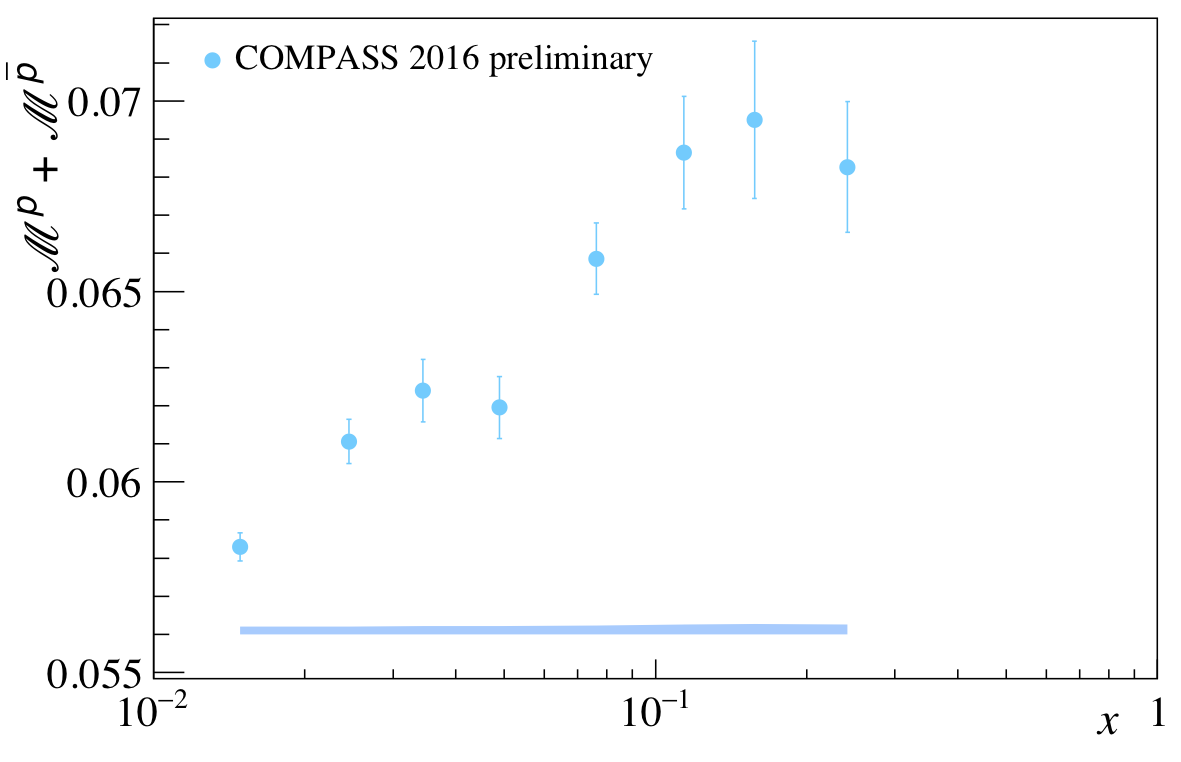
\includegraphics[scale=0.55]{./gfx/Ps.png}
	\caption{$\mathscr{M}^{p}+\mathscr{M}^{\bar{p}}$ versus $x$ for \textit{COMPASS} data (proton in blue  closed points) averaged over $y$ (0.1 to 0.7) and integrated over $z$ (0.2 to 0.85). All systematic errors are shown point to point as a band.}
	\label{Ps}
\end{figure}

\begin{figure}[H]
	\centering
	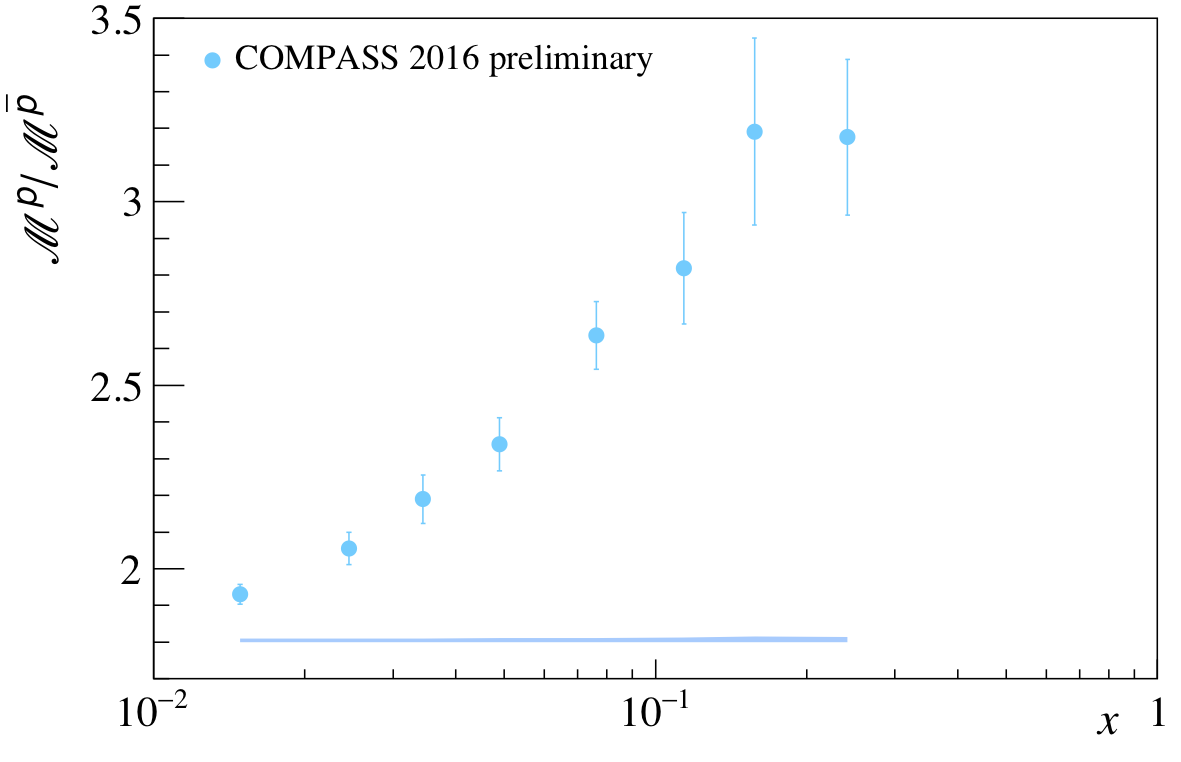
\includegraphics[scale=0.55]{./gfx/Pr.png}
	\caption{$\mathscr{M}^{p}/\mathscr{M}^{\bar{p}}$ versus $x$ for \textit{COMPASS} data (proton in blue closed points) averaged over $y$ (0.1 to 0.7) and integrated over $z$ (0.2 to 0.85). All systematic errors are shown point to point as a band.}
	\label{Pr}
\end{figure}

\newpage

\section{Release Material} \label{RM}

\begin{figure}[H]
	\centering
	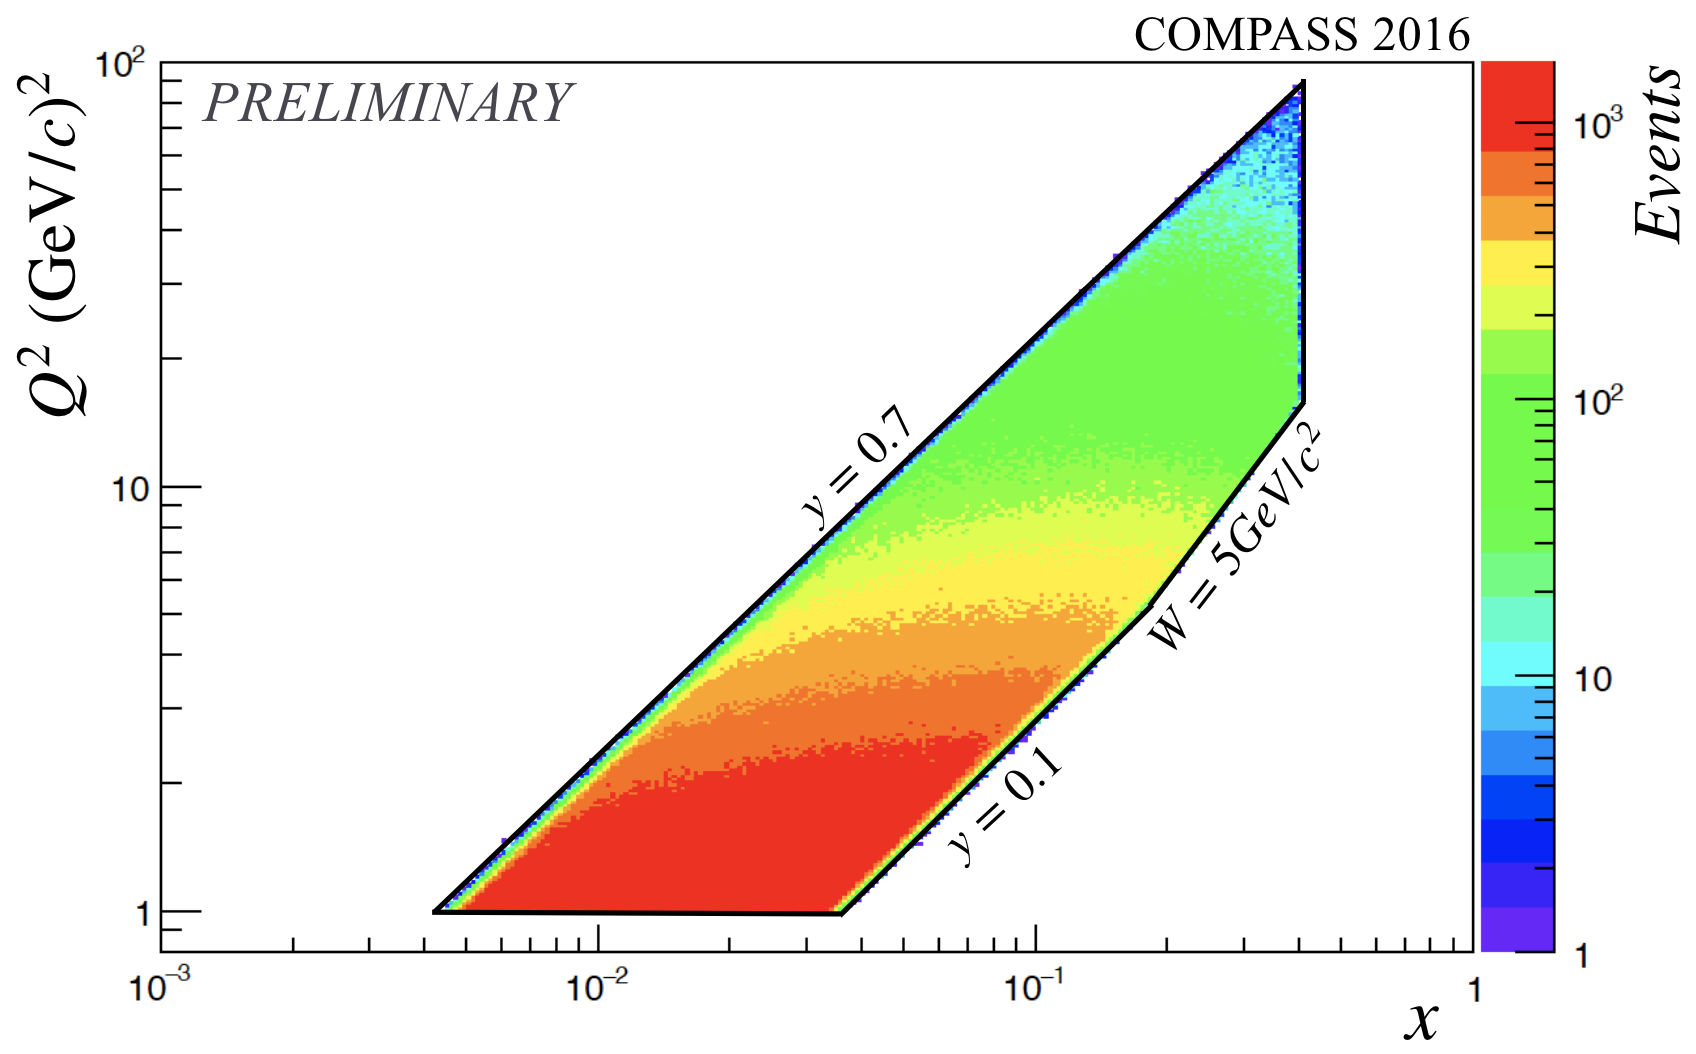
\includegraphics[scale=0.32]{./gfx/xQ2.png}
	\caption{Scatter-plot showing the $x$-$Q^2$ correlation of all DIS events selected for the current analysis for period between P07 and P11.}
	\label{xQ2}
\end{figure}

\begin{figure}[H]
	\centering
	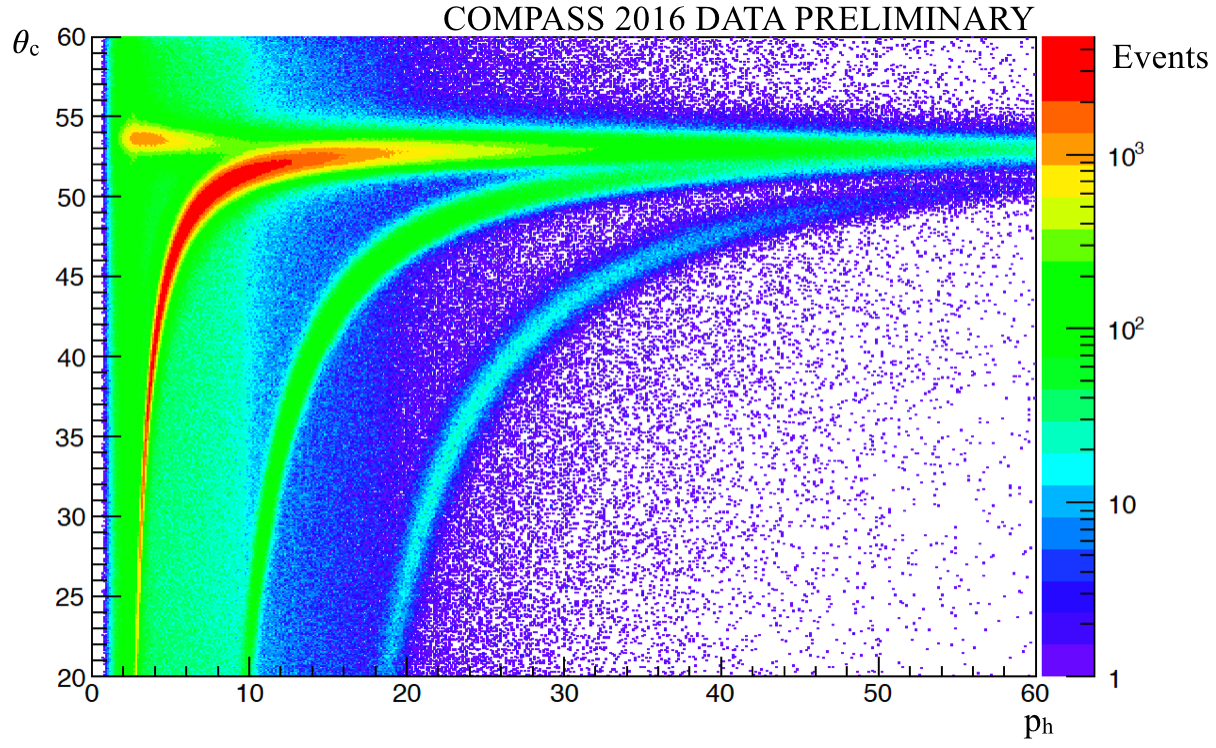
\includegraphics[scale=0.32]{./gfx/RICH.png}
	\caption{Scatter-plot showing the $p_h$-$\theta_c$ of hadrons in the RICH. There is a clear separation between $\pi$, $K$ and $p$ between 12 and 40 GeV/c.}
	\label{RICH}
\end{figure}

\begin{sidewaysfigure}[!p]
	\centering
	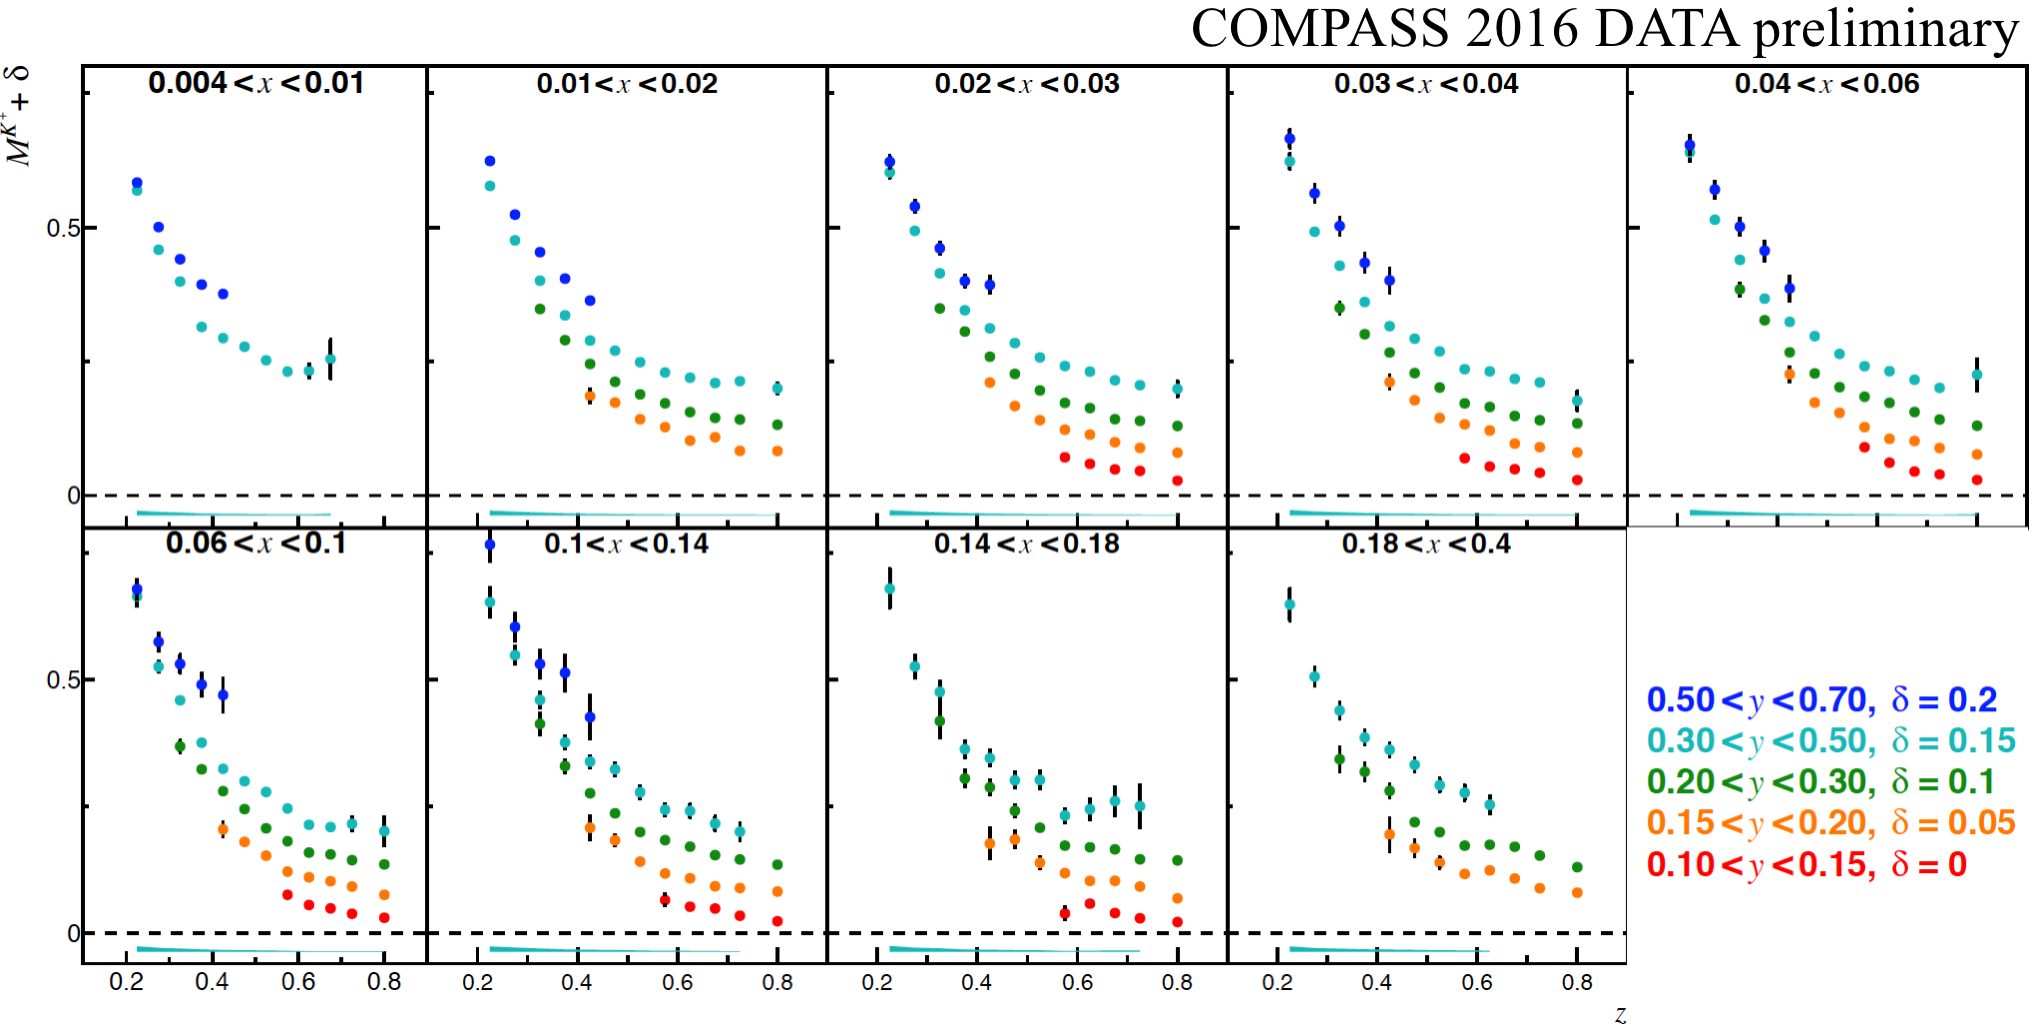
\includegraphics[scale=0.5]{./gfx/Kp.png}
	\caption{Final positive kaon multiplicities as a function of $z$ in bins of $x$ and staggered vertically with $y$. Radiative correction, diffractive vector meson correction and acceptance correction have been applied. All systematic errors are shown in band for the bin 0.3 $< y <$ 0.5.}
	\label{Kp}
\end{sidewaysfigure}

\begin{sidewaysfigure}[!p]
	\centering
	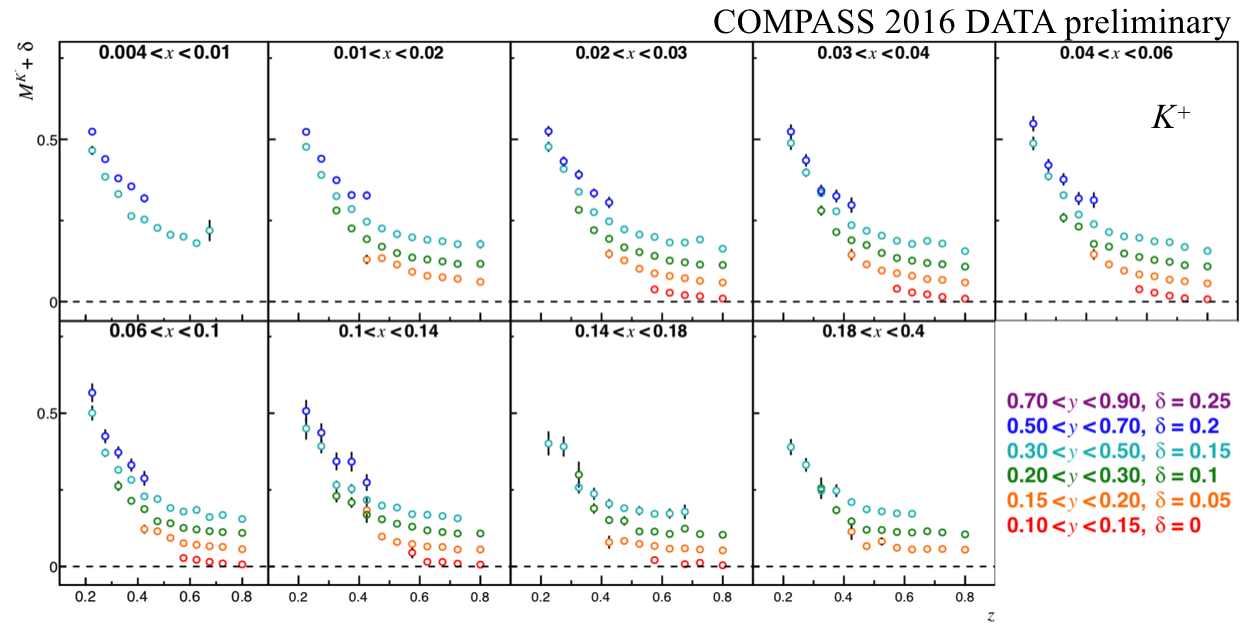
\includegraphics[scale=0.5]{./gfx/Km.png}
	\caption{Final negative kaon multiplicities as a function of $z$ in bins of $x$ and staggered vertically with $y$. Radiative correction, diffractive vector meson correction and acceptance correction have been applied. All systematic errors are shown in band for the bin 0.3 $< y <$ 0.5.}
	\label{Km}
\end{sidewaysfigure}

\newpage

\begin{figure}[H]
	\centering
	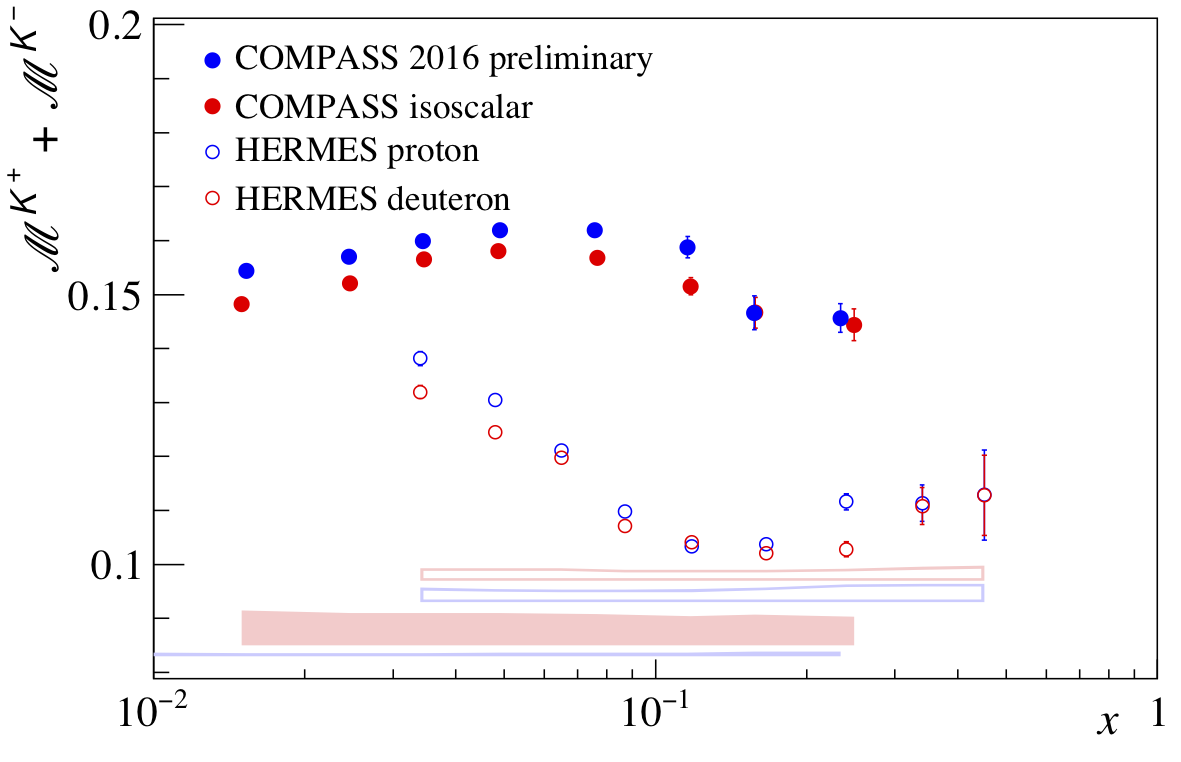
\includegraphics[scale=0.55]{./gfx/Ks.png}
	\caption{$\mathscr{M}^{K^+}+\mathscr{M}^{K^-}$ versus $x$ for \textit{COMPASS} data (proton in blue and isoscalar in red, closed points) averaged over $y$ (0.1 to 0.7) and integrated over $z$ (0.2 to 0.85) and \textit{HERMES} data \cite{HERMES} (proton in blue and deuteron in red, open points) averaged over $y$ (0.1 to 0.85) and integrated over $z$ (0.2 to 0.8). All systematic errors, including the asymmetric systematic errors for radiative correction for \textit{COMPASS} isoscalar kaons (100\% error, determined by removing the hadronic radiative corrections), are shown point to point as a band.}
	\label{Ks}
\end{figure}

\begin{figure}[H]
	\centering
	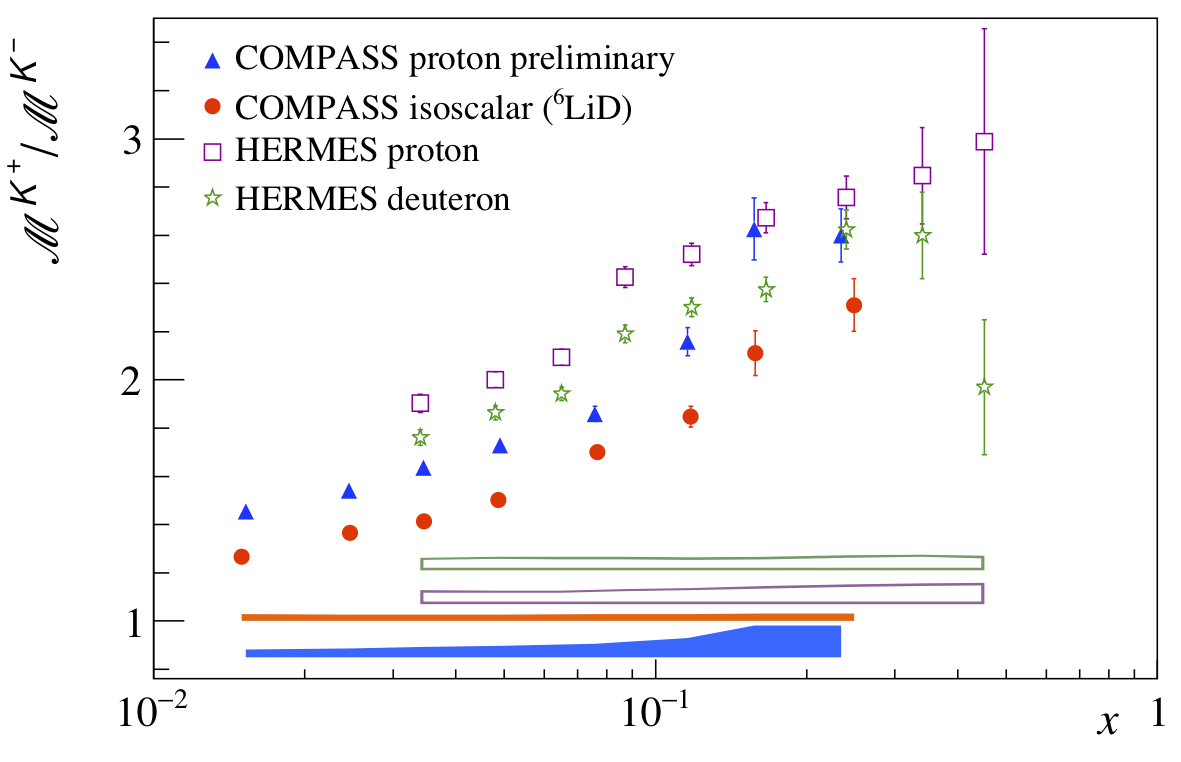
\includegraphics[scale=0.55]{./gfx/Kr.png}
	\caption{$\mathscr{M}^{K^+}/\mathscr{M}^{K^-}$ versus $x$ for \textit{COMPASS} data (proton in blue and isoscalar in red, closed points) averaged over $y$ (0.1 to 0.7) and integrated over $z$ (0.2 to 0.85) and \textit{HERMES} data \cite{HERMES} (proton in blue and deuteron in red, open points) averaged over $y$ (0.1 to 0.85) and integrated over $z$ (0.2 to 0.8). All systematic errors, including the asymmetric systematic errors for radiative correction for \textit{COMPASS} isoscalar kaons (100\% error, determined by removing the hadronic radiative corrections), are shown point to point as a band.}
	\label{Kr}
\end{figure}

\appendix

\section{Crosscheck} \label{XC}

\subsection{Data}

A crosscheck of the DIS selection, hadrons selection, RICH PID, unfolding and binning as well as the final multiplicities for pions, kaons and protons in bins of $x$, $y$ and $z$ over the full 5 weeks of data was done between Marcin and Nicolas. The crosscheck is yet to be finished but the agreement is found to the hadron after unfolding for the data.
% While for the cut flow, the agreement was perfect, the discrepancy on the final multiplicities is shown in a pull in Fig.\ref{}.
% In the figure, each entry is given by :

% \begin{equation}
% 	pull_i = \frac{M_i^{Nicolas}-M_i^{Marcin}}{\sigma_i^{Nicolas}}
% \end{equation}

% with $i$ being a given ($x$,$y$,$z$,$charge$) bin.

\subsection{MC}

A crosscheck between Marcin and Nicolas was performed. The crosscheck is yet to be finished but the agreement is found to the hadron after unfolding for the MC sample considered.
% The final acceptance in bins of $x$, $y$ and $z$ was found in perfect agreement.

\section{Error propagation} \label{Eprop}

This section explicitly describes the statistical error propagation used in the multiplicity calculation. Looping through DIS events, the squared error is :

\begin{equation}
		E^2_{DIS} = 1
\end{equation}

Looping through unidentified hadrons, the squared error is :

\begin{equation}
		E^2_{Had} = 1
\end{equation}

For identified hadrons, the squared error includes the RICH statistical error :

\begin{equation}
		E^2_{Had} = E^2_{RICH}
\end{equation}

where from Section \ref{Sys} :

\begin{equation}
		E^2_{RICH}[0<h<3] = cov(M^{-1}_{hr},M^{-1}_{hr})+(M^{-1}_{hr})^2
\end{equation}

with $M_{hr}$ the element of the RICH unfolding matrix for hadron $h$ from RICH identified hadron $r$ and :

\begin{equation}
		cov(M^{-1}_{hr},M^{-1}_{hr}) = \sum_{0<i,j,k,l<3} M^{-1}_{hi}M^{-1}_{jr}M^{-1}_{hk}M^{-1}_{lr}cov(M_{ij},M_{kl})
\end{equation}

For the raw multiplicities the error takes into account the correlation between hadrons and DIS events :

\begin{equation}
		E^2_{raw} = \Bigg[\frac{E^2_{Had}}{N^2_{DIS}} - \bigg( \frac{N^2_{Had}}{N^2_{DIS}} \bigg)^2 E^2_{DIS} \Bigg]/z^2_{width}
\end{equation}

For the acceptance correction (Section \ref{Cor}) the covariance between the DIS events and hadrons is not considered and the acceptance is treated as 2 independent quasi-binomial distributions :

\begin{equation}
\begin{split}
		E^2_{acc} = \bigg(\frac{G_D}{R_D+R_{D'}}\bigg) \bigg[ \frac{\big( R_h+1 \big)\big( G_h-R_h+1 \big)}{\big( G_h+2 \big)^2\big( G_h+3 \big)}+\frac{R'_h}{G^2_h}+\frac{R'^2_h}{G^3_h} \bigg] \\
		+ \bigg(\frac{G_D}{R_D+R_{D'}}\bigg)^4 \bigg(\frac{R_h+R'_h}{G_h}\bigg)^2 \bigg[ \frac{\big( R_D+1 \big)\big( G_D-R_D+1 \big)}{\big( G_D+2 \big)^2\big( G_D+3 \big)}+\frac{R'_D}{G^2_D}+\frac{R'^2_D}{G^3_D} \bigg]
\end{split}
\end{equation}

where $G_h$ (resp. $G_D$) are the generated hadrons (resp. DIS events) in a given $x$, $y$, $z$ bin, $R_h$ (resp. $R_D$) the reconstructed hadrons (resp. DIS events) and $R'_h$ (resp. $R'_D$) all other particles (resp. events) that are reconstructed as hadrons (resp. DIS events) in a given $x$, $y$, $z$ bin.

Finally for the multiplicity, including the diffractive $\Phi$ and $\rho^0$ correction error ($E_{VM}$) and radiative correction error ($E_{RC}$):

\begin{equation}
\begin{split}
		E^2_{Final} = \bigg( \frac{RC.VM}{Acc} \bigg)^2 E^2_{Raw} + \bigg(\frac{RC.VM.Raw}{Acc^2} \bigg)^2 E^2_{Acc} \\
		+ \bigg(\frac{RC.Raw}{Acc} \bigg)^2 E^2_{VM} + \bigg(\frac{VM.Raw}{Acc} \bigg)^2 E^2_{RC}
\end{split}
\end{equation}

%++++++++++++++++++++++++++++++++++++++++
% References section will be created automatically
% with inclusion of "thebibliography" environment
% as it shown below. See text starting with line
% \begin{thebibliography}{99}
% Note: with this approach it is YOUR responsibility to put them in order
% of appearance.

\newpage

\begin{thebibliography}{99}

\bibitem{JanPt}
F. Bradamante, A. Bressan, A. Kerbizi, J. Matousek, A. Moretti, A. Martin and A. Ivanov, \textit{Release note on PhT-dependent charged hadron multiplicities from 2016 data}, COMPASS Release Note April 2019.

\bibitem{COMPASS2006P}
C. Adolph et al., \textit{Multiplicities of charged pions and unidentified charged hadrons from deep-inelastic scattering of muons off an isoscalar target}, PLB 763 (2017) 001.

\bibitem{COMPASS2006K}
C. Adolph et al., \textit{Multiplicities of charged kaons from deep-inelastic muon scattering off an isoscalar target}, PLB 763 (2017) 133.

\bibitem{DJANGOH_NOTE}
N. Pierre, \textit{DJANGOH : a Monte-Carlo Generator with Radiative Corrections}, COMPASS Note 2018-3.

\bibitem{RICH_NOTE}
M. Wilfert and J. Giarra, \textit{RICH performance in 2011/12}, COMPASS Note 2017-6.

\bibitem{Release2015}
Y. Bedfer, N. du Fresne, D. Hahne, N. Pierre, E. Seder, M. Stolarski, V. Andrieux, L. Capozza, Q. Curiel, F. Thibaud, E. Kabu{\ss}, F. Kunne, N. Makke, C. Marchand, F. Sozzi, \textit{Charged kaon multiplicities from muon deep inelastic scattering on $^6$LiD (2006 COMPASS data)}, COMPASS Release Note May 2015.

\bibitem{Goloskokov}
S. V. Goloskokov and P. Kroll, \textit{The role of the quark and gluon GPDs in hard vector-meson electroproduction}, arXiv:0708.3569 [hep-ph].

\bibitem{Hepgen}
A. Sandacz and P. Sznajder, \textit{HEPGEN - generator for hard exclusive leptoproduction}, arXiv:1207.0333 [hep-ph].

\bibitem{HERMES}
A. Airapetian et al., \textit{Multiplicities of charged pions and kaons from semi-inclusive deep-inelastic scattering by the proton and the deuteron}, Phys.Rev. D87 (2013) 074029.

\end{thebibliography}


\end{document}
